\documentclass{article}
\usepackage{times}
\usepackage{graphicx}
\usepackage{subfigure} 
\usepackage{natbib}
\usepackage{algorithm}
\usepackage{amsmath}
\usepackage{amsthm}%For stating numbered theorems
\usepackage{amsfonts}
\usepackage{algorithmic}
\usepackage{subfigure}
\usepackage{hyperref}
\newcommand{\theHalgorithm}{\arabic{algorithm}} % Fixes misbehavior of conflicting packages.
\usepackage{icml2016/icml2016} 
\usepackage[nolist]{acronym} % Acronym package -- give argument <dua> to suppress acronym usage

%Theorem declarations
\newtheorem{thm}{Theorem}
\newtheorem{lma}{Lemma}
\newtheorem{clm}{Claim}

\newtheoremstyle{dotless}{}{}{\itshape}{}{\bfseries}{}{ }{}
\theoremstyle{dotless}
\newtheorem{defn}{Definition}

\newcommand{\bdefn}[1]{
\begin{defn} {\boldmath, #1}\textbf{:}
}

\newcommand{\edefn}[1]{
\end{defn}
}

\icmltitlerunning{Near Optimal Behavior with Approximate State Abstraction}

% --- Notation Commands ---
\newcommand{\ep}{\widetilde \phi}
\newcommand{\epQ}{\ep_{Q^*}}
\newcommand{\epM}{\ep_{\text{model}}}
\DeclareMathOperator*{\argmin}{arg\,min}
\DeclareMathOperator*{\argmax}{arg\,max}
\newcommand{\mc}[1]{\mathcal{#1}}
\newcommand{\mcS}{\mathcal{S}}
\newcommand{\mcT}{\mathcal{T}}
\newcommand{\mcR}{\mathcal{R}}
\newcommand{\pM}{\phi_{\text{model}}}


% --- Note Commands ---
\usepackage{color}
\newcommand\dnote[1]{\textcolor{blue}{Dave: #1}}
\newcommand\enote[1]{\textcolor{green}{Ellis: #1}}

% --- DOCUMENT ---
\begin{document}

\twocolumn[
% Suboptimality Bounds for Approximate State Abstraction
\icmltitle{Near Optimal Behavior with Approximate State Abstraction}

% Paper Meta Info
\icmlauthor{David Abel}{david_abel@brown.edu}
\icmladdress{Brown University,
            115 Waterman Street, Providence, RI 02906}
\icmlauthor{D. Ellis Hershkowitz}{david_hershkowitz@brown.edu}
\icmladdress{Brown University,
            115 Waterman Street, Providence, RI 02906}
\icmlauthor{Michael L.\ Littman}{michael_littman@brown.edu}
\icmladdress{Brown University,
            115 Waterman Street, Providence, RI 02906}
    
\icmlkeywords{Reinforcement Learning, State Aggregation, State Abstraction, Planning, MDP}
            
\vskip 0.3in
]

%Acronyms -- use \ac for acronym or \acp for plural/capitalization of acronym
\begin{acronym}
\acro{MDP}{Markov Decision Process}
\acrodefplural{MDP}[MDPs]{Markov Decision Processes}
\acro{RL}{reinforcement learning}
\acrodefplural{RL}{Reinforcement learning}
\end{acronym}


% ------------------------
% --- ABSTRACT ---
% ------------------------
\begin{abstract}
The combinatorial explosion that plagues planning and \ac{RL} algorithms can be moderated using abstraction. Prohibitively difficult task representations can be condensed such that essential information is preserved, and consequently, solutions are tractably computable. However, perfect abstractions are often computationally intractable and ineffective in environments where no two situations are exactly alike. For these reasons, we investigate approximate abstractions, which treat nearly-identical situations as equivalent. In this work, we characterize sufficient conditions for approximate abstractions that preserve near optimal behavior while reducing the complexity of the original task representation. We present theoretical guarantees of the quality of behaviors derived from four classes of approximate abstractions. Additionally, we empirically demonstrate that approximate abstractions lead to reduction in task complexity and bounded loss of optimality of behavior in a variety of environments. % Environments could also be tasks/problems/etc

%as approximations become tighter, 
% as knowledge becomes more approximate.


% Old one:
% Abstraction plays a fundamental role in learning. Through abstraction, intelligent agents may reason about only the salient features of their environment while ignoring what is irrelevant, consequently enabling agents to solve considerably more complex problems. However, in natural environments, no two states are identical. This work characterizes the impact of combining ``sufficiently similar'' states in the context of planning and \ac{RL} in \acp{MDP}.


%Because of the difficulty of acquiring perfect knowledge, agents must often perform approximate abstraction on the basis of incomplete knowledge.




% There are a variety of attractive characteristics of approximate abstractions.

%decreasing with degrees of incompleteness of knowledge in a variety of \acp{MDP}.
%
%reduction in task complexity at the cost of bounded increase in error of behavior.
%
%that the relationship between the degree of approximation and the degree of  achieved in a variety of example tasks, as well as the tradeoff between the degree of approximation and the optimality of behavior.

%that achieves high degrees of compression while preserving near optimal behavior
%In this work, we investigate a theory of approximate state abstraction that achieves high degrees of compression while preserving near optimal behavior.




% We fight exponentials with abstraction.
\end{abstract}


% ---------------------------------------
% --- SECTION: Introduction ---
% ---------------------------------------
\section{Introduction}
Abstraction plays a fundamental role in learning. Through abstraction, intelligent agents may reason about only the salient features of their environment while ignoring what is irrelevant. Consequently, agents are able to solve considerably more complex problems than they would be able to without the use of abstraction. However, \textit{exact abstractions}, which treat fully-identical situations alike, require complete knowledge that is often computationally intractable to obtain. Furthermore, often no two situations are identical, so exact abstractions are often ineffective. To overcome these issues we investigate \textit{approximate abstractions} that enable agents to treat sufficiently similar situations as identical. This work characterizes the impact of equating ``sufficiently similar'' states in the context of planning and \ac{RL} in \acp{MDP}. The remainder of our introduction contextualizes these intuitions in \acp{MDP}.

% Abstraction is a good idea b/c MDP has poly comp comp and samp comp in S, but S grows fast.
Solving for optimal behavior in \acp{MDP} in a planning setting is known to be P-Complete in the size of the state space~\cite{papadimitriou1987complexity,littman1995complexity}. Similarly, many \ac{RL} algorithms for solving \acp{MDP} are known to require a number of samples polynomial in the size of the state space~\cite{strehl2009reinforcement}. Although polynomial runtime or sample complexity may seem like a reasonable constraint, the size of the state space of an \ac{MDP} grows super-polynomially with the number of variables that characterize the domain, a results of Bellman's curse of dimensionality. Thus, solutions polynomial in state space size are often ineffective for sufficiently complex tasks. \dnote{Would prefer a different example} For instance, a robot involved in a pick and place task might be able to employ planning algorithms to solve for how to manipulate some objects into a desired configuration in time polynomial in the number of states, but the number of states it must consider to do so grows exponentially with the number of objects it plans over \enote{Cite Dabe Icaps}.

% Existing work on state abstraction.
Thus, a key research agenda for planning and \ac{RL} is leveraging abstraction to reduce large state spaces~\cite{andre2002state,jong2005state,dietterich2000hierarchical,Bean2011}. This agenda has given rise to methods that reduce \textit{ground} \acp{MDP} with large state spaces to \textit{abstract} MDPs with smaller state spaces by aggregating states according to some notion of equality or similarity. In the context of \acp{MDP}, we understand exact abstractions as those that aggregate states with equal values of particular quantities, e.g. optimal $Q$-values. Existing work has characterized how exact abstractions can fully maintain optimality in \acp{MDP}~\cite{li2006towards,dean1997modelmin}. 

% Thesis: Approximate abstraction for three reasons.
Performing approximate abstraction in \acp{MDP} by relaxing the state aggregation criteria from equality of quantities to $\epsilon$-closeness offers three benefits. First, approximate abstractions employ the sort of knowledge that we expect a planning or learning algorithm to compute without fully solving the \ac{MDP}. In contrast, exact abstractions often require solving for optimal behavior, thereby defeating the purpose of abstraction. Second, because of their relaxed criteria, approximate abstractions can achieve greater degrees of compression than exact abstractions. This difference is particularly important in environments where no two states are identical. \dnote{note this in empirical results discussion, that random is sort of like a natural environment and when eps is 0, no compression} Third, because the state aggregation criteria are relaxed to approximate equality, approximate abstractions are able to tune the aggressiveness of abstraction by adjusting what they consider sufficiently similar states. The thesis of this work is that aggregation of states on the basis of various approximate criteria can reduce state space size while incurring only bounded error in the resulting behavior.

% Summary	
This paper is organized as follows. We first introduce the necessary terminology and background of \acp{MDP} and state abstraction. We then survey existing types of state abstraction as applied to sequential decision making. The following section introduces our primary result; bounds on the error guaranteed by four classes of approximate state abstraction. We then discuss experiments in which we apply one class of approximate abstraction to a variety of different tasks, visualizing the abstractions and showing the relationship between degree of compression and error incurred.



% ---------------------------------------
% --- SECTION: Background ---
% ---------------------------------------

\section{Background}

%First, some background.

zzz: I think empty sections like this are ugly. There ought to be some sort of preamble here.

%MDP/SDM Background and Notation
\subsection{\acp{MDP} and Sequential Decision Making}
\enote{Come back to this and make sure it covers everything that needs to be covered and matches all our notation.}
An \ac{MDP} is a problem representation for sequential decision making agents, represented by a five-tuple: $\langle \mathcal{S}, \mathcal{A}, \mathcal{T}, \mathcal{R}, \gamma \rangle$. Here, $\mathcal{S}$ is a finite state space; $\mathcal{A}$ is a finite set of actions available to the agent; $\mathcal{T}$ denotes $\mathcal{T}(s' \mid s,a)$, the probability of an agent transitioning to state $s' \in \mathcal{S}$ after applying action $a \in \mathcal{A}$ in state $s \in \mathcal{S}$; $\mathcal{R}(s,a)$ denotes the reward received by the agent for executing action $a$ in state $s$; $\gamma \in [0, 1]$ is a discount factor that determines how much the agent prefers future rewards over immediate rewards. We assume without loss of generality that the range of all reward functions is normalized to $[0,1]$. The solution to an \ac{MDP} is called a policy, denoted $\pi: \mathcal{S} \mapsto \mathcal{A}$.

The objective of an agent is to solve for the policy that maximizes its expected discounted reward from any state, denoted $\pi^*$. We denote the expected discounted reward for following policy $\pi$ from state $s$ as the value of the state under that policy, $V^\pi(s)$. We similarly denote the expected discounted reward for taking action $a \in \mathcal{A}$ and then following policy $\pi$ from state $s$ forever after as $Q^\pi(s,a)$, defined by the Bellman Equation as:
\begin{equation}
Q^\pi(s,a) = \mathcal{R}(s,a) + \gamma \sum_{s'} \mathcal{T}(s,a,s') Q^\pi(s',\pi(s)).
\end{equation}
Similarly, the value function defined under a given policy, denoted $V^\pi(s)$, is defined as:
\begin{equation}
V^\pi(s) = \max_a Q^\pi(s,a).
\end{equation}

zzz no, that is not the standard definition. it would normally be $V^\pi(s) = Q^\pi(s,\pi(s))$.

Lastly, we denote the value and $Q$ functions under the optimal policy as $V^*$ or $V^{\pi^*}$ and $Q^*$ or $Q^{\pi^*}$, respectively. For further background, see~\namecite{kaelbling1996reinforcement}.

%Lihong Section
\subsection{Abstraction Notation}
We build upon the notation used by \citeauthoryear{li2006towards}, who introduced a unifying theoretical framework for state abstraction in \acp{MDP} and sequential decision making. We build heavily on their notation, and discuss other similarities to our work in the next section.

\bdefn{$M_G$, $M_A$}
We understand an abstraction as a mapping from the state space of a ground MDP $M_G$ to that of an abstract MDP $M_A$ using a state-aggregation scheme. Consequently, this mapping induces an abstract MDP. Let $M_G = \langle \mathcal{S}_G, \mathcal{A}, \mathcal{T}_G, \mathcal{R}_G, \gamma \rangle$ and $M_A = \langle \mathcal{S}_A, \mathcal{A}, \mathcal{T}_A, \mathcal{R}_A, \gamma \rangle$.
\edefn

% States
\bdefn{$\mcS_A$, $\phi$}
The states in the abstract \ac{MDP} are constructed by applying a state-aggregation function, $\phi$, to the states in the ground \ac{MDP}, $\mathcal{S}_A$. More specifically, $\phi$ maps a state in the ground \ac{MDP} to a state in the abstract \ac{MDP}:
\begin{equation}
\mathcal{S}_A = \{ \phi(s) \mid s \in \mathcal{S}_G\}.
\end{equation}
\edefn

zzz the space before the comma looks weird to me.

\bdefn{$G$}
Given a $\phi$, each ground state has associated with it the ground states with which it is aggregated. Similarly, each abstract state has its constituent ground states. We let $G$ be the function that retrieves these states:
\begin{equation}
G(s)=
\begin{cases}
\{g \in \mcS_G \mid \phi(g) = \phi(s) \},& s \in \mcS_G,\\
\{g \in \mcS_G \mid \phi(g)=s \},& s \in \mcS_A.
\end{cases}
\end{equation}
\edefn

The abstract reward function and abstract transition dynamics for each abstract state are a weighted combination of the rewards and transitions for each ground state in the partition. We make no assumptions about the weighting scheme, except that for each abstract state, the weighting is a convex combination across all ground states.

zzz it's weird that s is bound twice in this formula. is that needed/intentional?

\bdefn{$\omega(s)$}
We refer to the weight associated with a ground state, $s \in \mathcal{S}_G$ by $\omega(s)$. The only restriction placed on the weighting scheme is that it induces a probability distribution on the states:
\begin{equation}
\forall s \in \mcS_G \left(\sum_{s \in G(s)} \omega(s)\right) = 1 \textrm{ and }\hspace{6mm}  \omega(s) \in [0,1].
\end{equation}
\edefn

% Reward
\bdefn{$\mcR_A$}
The abstract reward function $\mathcal{R}_A(s,a)$ is a weighted sum of the rewards of each of the ground states that map to the same abstract state:
\begin{equation}
\mathcal{R}_A(s,a) = \sum_{g \in G(s)} \mathcal{R}_G(g,a) \omega(g) .
\end{equation}
\edefn

% Transition
\bdefn{$\mcT_A$}
The abstract transition function $\mathcal{T}_A(s,a,s')$ is a weighted sum of the transitions of each of the ground states that map to the same abstract state:
\begin{equation}
\mathcal{T}_A(s,a,s') = \sum_{g \in G(s)} \sum_{g' \in G(s')} \mathcal{T}_G(g,a,g') \omega(g).
\end{equation}
\edefn



%\enote{Define $V_G$ and $V_A$ (value function in ground and value function in abstract)}
%\dnote{This should be done in the background section, right? Just defining a value fund under a policy}

% Subsection: Exact Abstraction Framework












% -----------------------------------------
% --- SECTION: Related Work ---
% -----------------------------------------
\section{Related Work}

Several other projects have addressed similar topics.

\subsection{Approximate State Abstraction}
\citet{dean1997model} investigated partitioning an \ac{MDP}'s state space into $\varepsilon$-homogenous blocks, which are defined as clusters of states whose transition model and reward function are within $\varepsilon$ of each other. They develop an algorithm called Interval Value Iteration (IVI) that converges to the correct bounds on a family of abstracted MDPs called a Bounded MDP. This method of abstraction is effectively characterized as a function belonging to the approximate class $\phi_{model}$.
Several approaches build on the notion of $\varepsilon$-homogeneity. \citet{even2003approximate} analyzed different distance metrics used in the process of identifying $\varepsilon$-homogenous partitions. \citet{ortner2013adaptive} developed an algorithm for learning partitions in an online setting by taking advantage of the confidence bounds for $\mcT$ and $\mcR$ provided by UCRL~\cite{auer2009near}.

\subsection{Specific Abstraction Algorithms}
Many previous works have targeted the creation of algorithms that enable state abstraction for MDPs. \citet{andre2002state} investigated a method for state abstraction in hierarchical reinforcement learning leveraging a programming language called ALISP that promotes the notion of {\it safe} state abstraction. Agents programmed using ALISP can ignore irrelevant parts of the state, achieving abstractions that maintain optimality. \citet{dietterich2000hierarchical} developed MAXQ, a framework for composing tasks into an abstracted hierarchy where state aggregation can be applied. \citet{jong2005state} introduced a method called {\it policy-irrelevance} in which agents identify (online) which state variables may be safely abstracted away in a factored-state \ac{MDP}. The agent will learn to ignore state variables that don't impact optimal behavior. For a more complete survey of algorithms that leverage state abstraction in past reinforcement-learning papers, see \citet{li2006towards}.

\subsection{Exact Abstraction Framework}

\citet{li2006towards} developed a framework for exact state abstraction in \acp{MDP}. In particular, the authors defined five classes of state-aggregation functions, inspired by existing methods for state aggregation in \acp{MDP}. We generalize two of these five classes, $\phi_{Q^*}$ and $\phi_{\text{model}}$, to the approximate abstraction case. Note that when $\varepsilon=0$ our generalizations are equivalent to the corresponding exact methods. Additionally, when $\varepsilon=0$ our bounds indicate that no value is lost, which is one of core results of \citet{li2006towards}.

%zzz you shouldn't have $\phi_{model}$ because the word model will be typeset as the product of five variables. Some math mode magic is needed.




% ----------------------------------------------------------------
% --- SECTION: Approximate State Abstraction  ---
% ----------------------------------------------------------------
% --- SECTION: State Abstraction ---
\section{Approximate State Abstraction}

% Intro to approx state abstraction results.
Here, we introduce our formal method for analyzing approximate state abstraction, including results bounding the error associated with these abstraction methods. In particular, we demonstrate that abstractions based on approximate $Q^*$ similarity (\ref{sec:Q*}), approximate model similarity (\ref{sec:model}), and approximate similarity between distributions over $Q^*$, for both Boltzmann (\ref{sec:boltz}) and multinomial (\ref{sec:mult}) distributions, induce abstract \acp{MDP} for which the optimal policy has bounded error in the ground MDP.

%In general, our proof strategy for each of the included results is as follows:
%\begin{itemize}
%\item First, we relate the values of states in the ground MDP to the value of states in the abstract \ac{MDP},
%\item then, we relate the value of states in the ground \ac{MDP} to the value of states in the abstract \ac{MDP} under the optimal abstract policy.
%\end{itemize}

% Explanation of the above.
%The first statement is relating Q values defined over the ground MDP with Q values defined over the abstract MDP, while the second statement is comparing the optimal Q values in the ground MDP, with the Q values in the ground MDP under the abstract policy. This is because our learners will solve for the optimal policy in the abstract, and use it in the ground MDP by mapping each ground state to its abstract state and querying the abstract policy for behavior. That is:
%\begin{equation}
%\pi_G(s) = \pi_A(\phi(s))
%\end{equation}


% zzz that's odd... sounds like the same thing twice but with optimal policy added. we'll see how that works.
% In response^^^ Could add a sentence pointing out how these differ.

We now introduce some additional notation to formally discuss these results.

\bdefn{$\pi_A^*$, $\pi_G^*$}
We let $\pi_A^* : \mcS_A \rightarrow \mcA$ and $\pi_G^* : \mcS_G \rightarrow \mcA$ stand for the optimal policies in the abstract and ground \acp{MDP} respectively.
\edefn

% Abstract policy in ground.
We are interested in how the optimal policy in the abstract \ac{MDP} performs in the ground \ac{MDP}. As such we formally define the policy in the ground \ac{MDP} derived from optimal behavior in the abstract \ac{MDP}:

\bdefn{$\pi_{GA}$}
Given a $s \in \mcS_G$ and a state aggregation function, $\phi$, 
\begin{equation}
\pi_{GA}(s)=\pi_A^*(\phi(s))
\end{equation}
\edefn

We now define classes of abstraction based on functions state, action pairs.
\bdefn{$\ep_f$}
Given a function $f: \mathcal{S}_G \times \mathcal{A} \rightarrow \mathcal{R}$ and a fixed non-negative $\epsilon \in \mathbb{R}$, we define $\ep_f$ as a type of approximate state-aggregation function that satisfies the following for any two ground states $s_1$ and $s_2$: 
\begin{equation}
\label{eq:phi_f}
\ep_f(s_1) = \ep_f(s_2) \rightarrow \forall_a \left|f(s_1, a) - f(s_2, a)\right| \leq \epsilon
\end{equation}
\edefn

That is, when $\ep_f$ aggregates states, all aggregated states have values of $f$ within $\epsilon$ of each other for all actions.

\bdefn{$Q_G$, $V_G$}
Let $Q_G = Q^{\pi_G^*} : \mathcal{S}_G \times \mathcal{A} \rightarrow \mathbb{R} $ and $V_G = V^{\pi_G^*}: \mathcal{S}_G \rightarrow \mathbb{R} $ denote the optimal Q and optimal value functions in the ground \ac{MDP}.
\edefn

\bdefn{$Q_A$, $V_A$}
Let $Q_A  = Q^{\pi_A^*}: \mathcal{S}_A \times \mathcal{A} \rightarrow \mathbb{R}$ and $V_A  = V^{\pi_A^*}: \mathcal{S}_A \rightarrow \mathbb{R}$  stand for the optimal Q and optimal value functions in the abstract \ac{MDP}.
\edefn

We now introduce the main result of the paper.

% Theorem 1
\begin{thm}
There exist at least four classes of approximate state-aggregation functions, $\ep_{Q^*}$, $\ep_{\text{model}}$, $\ep_{\text{bolt}}$ and $\ep_{\text{mult}}$ for which the optimal policy in the abstract \ac{MDP}, applied to the ground \ac{MDP}, has suboptimality bounded polynomially in $\epsilon$:
\begin{equation}
\forall_{s \in \mathcal{S}_G}: | V_G^{\pi_{GA}}(s) - V_G^{\pi_G^*}(s) | \leq poly(\epsilon).
\end{equation}
\end{thm}
\enote{Axe the absolute values here and elsewhere}

\enote{Unify the use of $\forall$ and ``:"s}

\enote{Add for 0-1 normalized reward}

\enote{Add note relating this all to Lihong for eps=0 and cut down the Lihong section}

% Subsection: Optimal Q Function
\subsection{Optimal Q Function: $\ep_{Q^*}$}
\label{sec:Q*}

% Q* Lemma -- lemma 1
We consider an approximate version of the $Q^*$-irrelevance abstraction. 

\bdefn{$\epQ$}
An approximate $Q$ function has the same form as Equation~\ref{eq:phi_f}:
\begin{equation}
\ep_{Q^*}(s_1) = \ep_{Q^*}(s_2) \rightarrow \forall_a \left|Q_G^*(s_1, a) - Q_G^*(s_2, a)\right| \leq \epsilon.
\end{equation}
\edefn

% Q^* Lemma
\begin{lma}
\label{lma:Q*}
When $\ep_{Q^*}$ is used to create the abstract state space $\mcS_A$:
\begin{equation}
\forall_{s \in \mcS_G}: | V_G^{\pi_G^*}(s) - V_G^{\pi_{GA}}(s) | \leq \frac{2\epsilon}{(1-\gamma)^2}.
\end{equation}
\end{lma}

% Proof
\textbf{Proof:}
\enote{I would like a quick overview of the proof here if nobody objects.}
% Claim 1:
\begin{clm}
\label{clm:closeQs}
Optimal $Q$ values in the abstract \ac{MDP} closely resemble optimal $Q$ values in the ground \ac{MDP}:
\begin{equation}
\label{eq:Q*Claim1}
\forall_{s_G \in \mathcal{S}_G, a} |Q_G(s_G, a) - Q_A(\epQ(s_G), a)| \leq \frac{\epsilon}{1-\gamma}.
\end{equation}
\end{clm}

Consider a temporally heterogeneous \ac{MDP}, $M^T = \langle \mathcal{S}_T, \mathcal{A}_G, \mathcal{R}_T, \mathcal{T}_T, \gamma \rangle$, parameterized by integer $T$, such that for the first $T$ time steps the reward function, transition dynamics and state space are those of the abstract MDP, $M_A$, and after $T$ time steps the reward function, transition dynamics and state spaces are those of the ground MDP, $M_G$. Thus,
\begin{equation}
\mathcal{S}_T = \begin{cases}
\mathcal{S}_G,& T \leq 0, \\
\mathcal{S}_A,& \text{o/w},
\end{cases}
\end{equation}
\begin{equation}
\mathcal{R}_T(s,a) = \begin{cases}
\mathcal{R}_G(s,a),& T \leq 0, \\
\mathcal{R}_A(s, a),& \text{o/w},
\end{cases}
\end{equation}
\begin{equation}
\mcT_T(s,a,s') = \begin{cases}
\mcT_G(s,a,s'),& T \leq 0, \\
\underset{{g \in G(s)}}{\sum}\left[w(g)\mcT_G(g, a, s')\right],& T = 1, \\
\mcT_A(s,a,s'),& \text{o/w}.
\end{cases}
\end{equation}

It follows that the $Q$-value of a state $s$ in $M^T$ for action $a$ is defined by:
% zzz too long... needs to be broken up.

\begin{equation}
Q_T(s, a) = 
\begin{cases}
	   Q_G(s, a) &  T=0\\
	   \underset{g \in G(s)}{\sum} \left[ w(g)Q_G(g,a) \right] & T = 1\\
	   \mathcal{R}_A(\epQ(s),a) + \sigma_{T-1}(s,a) &\text{o/w}

\end{cases}
\end{equation}

Where:
\begin{equation}
\sigma_{T-1}(s,a) = \gamma \underset{{s_A}' \in \mathcal{S}_A}{\sum} \mathcal{T}_A(\epQ(s),a,{s_A}') \max_{a'} Q_{T-1}({s_A}', a')
\end{equation}

We proceed by induction on $T$ to show that:
\begin{equation}
\forall_{T, s_G \in \mathcal{S}_G, a} |Q_G(s_G, a) - Q_T(s_G, a)| \leq \sum_{t=0}^{T-1} \epsilon \gamma^{t},
\end{equation}

% Base Case t=0
\textit{Base Case: $T = 0$}\\
When $T = 0$, $Q_T = Q_G$, so the result trivially follows.
% Base Case t=1
\textit{Base Case: $T = 1$}\\
\begin{align*}
&Q_1(s,a) = \underset{g \in G(s)}{\sum} \left[ w(g)Q_G(g,a) \right].
\end{align*}
Since all co-aggregated states have Q-values within $\epsilon$ of one another and $w(g)$ induces a convex combination,
\begin{align*}
&Q_1(s,a) \leq \epsilon \gamma^t + \epsilon + Q_G(s_G, a),\\
&Q_1(s,a) \leq \gamma\sum_{t=0}^{1} \epsilon \gamma^t + Q_G(s_G, a).
\end{align*}
Thus,
\begin{equation}
\left| Q_{1}(s_A, a) - Q_G(s_G,a) \right| \leq \gamma\sum_{t=0}^{1}\epsilon \gamma^t
\end{equation}
% Inductive Case
\textit{Inductive Case: $T > 1$}

We assume as our inductive hypothesis that:
\begin{equation}
\forall_{s_G \in \mathcal{S}_G, a} |Q_G(s_G, a) - Q_{T-1}(\epQ(s_G), a)| \leq \sum_{t=0}^{T-2} \epsilon \gamma^t.\\
\end{equation}

Consider a fixed but arbitrary state, $s_G \in \mathcal{S}_G$, and fixed but arbitrary action $a$.

We denote $\epQ(s_G)$ as $s_A$. 

By definition of $Q_{T}(s_A, a)$, $\mathcal{R}_A$, $\mathcal{T}_A$:

\begin{multline*}
Q_T(s_A, a) = \sum_{g \in G(s_A)}w(g)* \\ 
 \left[ R_0(g,a) + \gamma \sum_{g' \in \mathcal{S}_G} T_0(g,a,g') \max_{a'} Q_{T-1}(g', a')      \right]
\end{multline*}
Applying our inductive hypothesis yields,
\begin{multline*}
\leq \sum_{g \in G(s_A)}w(g) * \\ \left[ R_G(g,a) + \gamma \sum_{g' \in \mathcal{S}_G} T_G(g,a,g') \max_{a'}(Q_G(g', a') + \sum_{t=0}^{T-2} \epsilon \gamma^t)      \right]
\end{multline*}
%&\leq \gamma\sum_{t=0}^{T-2} \epsilon \gamma^t + \sum_{g \in X(s_A)}w(g)\left[ R_0(g,a) + \gamma \sum_{g' \in \mathcal{S}_G} T_0(g,a,g') \max_{a'}Q_0      \right]\\
Then:
\begin{equation*}
\leq \gamma\sum_{t=0}^{T-2} \epsilon \gamma^t + \sum_{g \in G(s_A)}\left[ w(g)\ Q_G(g,a)\right]
\end{equation*}
Since all aggregated states have Q-values within $\epsilon$ of one another:
\begin{align*}
&\leq \gamma\sum_{t=0}^{T-2} \epsilon \gamma^t + \epsilon + Q_G(s_G, a)\\
&\leq \gamma\sum_{t=0}^{T-1} \epsilon \gamma^t + Q_G(s_G, a)
\end{align*}
Thus,
\begin{equation*}
\left| Q_{T}(s_A, a) - Q_G(s_G,a) \right| \leq \gamma\sum_{t=0}^{T-1}\epsilon \gamma^t
\end{equation*}

Since $s_G$ and $s_A$ are arbitrary we conclude
\begin{equation}
\forall_{T, s_G \in \mathcal{S}_G, a} |Q_G(s_G, a) - Q_T(\epQ(s_G), a)| \leq \sum_{t=0}^{T-1} \epsilon \gamma^t
\end{equation}

As $T \rightarrow \infty$, $Q_T$ becomes $Q_A$ and $\sum_{t=0}^{T-1} \epsilon \gamma^t$ becomes $\frac{\epsilon}{1-\gamma}$. Therefore we conclude Equation $\ref{eq:Q*Claim1}$.



%Claim 2
\begin{clm}
\label{clm:optAbsActionNearOptGround}
The optimal action in the abstract MDP has a Q-value in the ground which is nearly optimal:

Consider a fixed but arbitrary state, $s_G \in \mathcal{S}_G$ and its corresponding abstract state $s_A=\epQ(s_G)$.

Let $a^*_G$ stand for the optimal action for $s_G$: \\
$a^*_G = \argmin Q_G(s_G, a)$

Let $a^*_A$ stand for the optimal action for $s_A$:\\
 $a^*_A = \argmin Q_A(s_A, a)$

That is, we prove that

\begin{equation}
\label{eq:Q*Claim2}
V_G(s_G) \leq Q_G(s_A, a^*_A) + \frac{2\epsilon}{1-\gamma}
\end{equation}
\end{clm}

By Claim \ref{clm:closeQs}
\begin{align}
&V_G(s_G) = Q_G(s_G, a^*_G) \leq Q_A(s_G, a^*_G) + \frac{\epsilon}{1-\gamma}
\label{eq:Q*OptActionResult}
\end{align}

 By the definition of $a^*_A$ we know that 
 \begin{align}
Q_A(s_G, a^*_G) + \frac{\epsilon}{1-\gamma} \leq Q_A(s_A, a^*_A) + \frac{\epsilon}{1-\gamma}
\end{align}

Lastly again by Claim \ref{clm:closeQs} we know
\begin{align}
Q_A(s_A, a^*_A) + \frac{\epsilon}{1-\gamma} \leq Q_G(s_A, a^*_A) + \frac{2\epsilon}{1-\gamma}
\end{align}

Therefore, we conclude Equation \ref{eq:Q*Claim2}.

%Claim 3
\begin{clm}
Lemma \ref{lma:Q*} follows from Claim \ref{clm:optAbsActionNearOptGround}.
\end{clm}

Consider the policy for $M_G$ of following the optimal abstract policy $\pi^*_A$ for t steps and then following the optimal ground policy $\pi^*_G$ in $M_G$:
\begin{equation}
\pi_{A,t}(s)=
\begin{cases}
\pi_G^*(s), \text{if $t<=0$}\\
\pi_{GA}(s), \text{if $t > 0$}
\end{cases}
\end{equation}

For a particular $t$, the value of this policy for $s_G \in \mathcal{S}_G$ in the ground \ac{MDP} is as follows:
\begin{multline*}
V_G^{\pi_{A,t}}(s_G) = \\
R_G(s, \pi_{A,t}(s_G)) +\ \gamma \sum_{{s_G}' \in \mathcal{S}_G}\mathcal{T}_G(s_G, a, {s_G}')V_G^{\pi_{A,t-1}}({s_G}')
\end{multline*}
%Start induction on following the optimal abstract policy
We now show by induction on $t$ that
\begin{equation}
\forall_{t, s_G \in \mathcal{S}_g} V_G(s_G) \leq  V_G^{\pi_{A,t}}(s_G) + \sum_{i=0}^{t}\gamma^i \frac{2\epsilon}{1-\gamma}
\end{equation}

\textit{Base case: $t=0$}

By definition when $t=0$, $V_G^{\pi_{A,t}} = V_G$ so our bound trivially holds in this case.

\textit{Inductive case: $t > 0$}

Consider a fixed but arbitrary state in $\mathcal{S}_G$, $s_G$.

We assume for our inductive hypothesis that
\begin{equation}
V_G(s_G) \leq V_G^{\pi_{A,t-1}}(s_G) + \sum_{i=0}^{t-1}\gamma^i \frac{2\epsilon}{1-\gamma}
\end{equation}
By definition 
\begin{multline*}
V_G^{\pi_{A,t}}(s_G) = R_G(s, \pi_{A,t}(s_G)) + \\ \gamma \sum_{g'}\mathcal{T}_G(s_G, a, {s_G}')V_G^{\pi_{A,t-1}}({s_G}')
\end{multline*}
Applying our inductive hypothesis yields:
\begin{multline*}
V_G^{\pi_{A,t}}(s_G, a) \geq R_G(s_G, \pi_{A,t}(s_G, a))\ + \\ \gamma \sum_{{s_G}'}\mathcal{T}_G(s_G, a, {s_G}')\left(V_G({s_G}') - \sum_{i=0}^{t-1}\gamma^i \frac{2\epsilon}{1-\gamma} \right)
\end{multline*}
Therefore:
\begin{align*}
%&\geq -\gamma\sum_{i=0}^{t-1}\gamma^i \frac{2\epsilon}{1-\gamma} + R_G(s, \pi_{A,t}(g)) + \gamma \sum_{g'}\mathcal{T}_G(g, a, g')V^{\pi^*}(g')\\
&\geq -\gamma\sum_{i=0}^{t-1}\gamma^i \frac{2\epsilon}{1-\gamma} + Q_G(s_G, \pi_{A,t} (s_G))
\end{align*}
Applying Claim \ref{clm:optAbsActionNearOptGround} yields:
\begin{align*}
&\geq \gamma\sum_{i=0}^{t-1}\gamma^i \frac{2\epsilon}{1-\gamma} - \frac{2\epsilon}{1-\gamma} + V_{G}(s_G)\\
&\leq \sum_{i=0}^{t}\gamma^i \frac{2\epsilon}{1-\gamma} + V_G(s_G)
\end{align*}

Thus,
\begin{equation*}
V_G(s_G) \leq V^{\pi_{A,t}}(s_G)  + \sum_{i=0}^{t}\gamma^i \frac{2\epsilon}{1-\gamma}
\end{equation*}
Since $s_G$ was arbitrary, we conclude that our bound holds for all states in $\mathcal{S}_G$ for the inductive case.

Thus, from our base case and induction we conclude that
\begin{equation}
\forall_{t, s_G \in \mathcal{S}_g} V^{\pi^*}(s_G) \leq  V^{\pi_{A,t}}(s_G) + \sum_{i=0}^{t}\gamma^i \frac{2\epsilon}{1-\gamma}
\end{equation}

Note that as $t \rightarrow \infty$, $\sum_{i=0}^{t}\gamma^i \frac{2\epsilon}{1-\gamma} \rightarrow \frac{2\epsilon}{(1-\gamma)^2}$ by the sum of geometric series and $\pi_{A,t}(s) \rightarrow \pi_{GA}$.

Thus, we conclude
\begin{equation*}
\forall_{s_G \in \mathcal{S}_g} V_G(s_G) \leq  V^{\pi_{GA}}(s_G) + \frac{2\epsilon}{(1-\gamma)^2}
\end{equation*}

\begin{equation*}
\forall_{s_G \in \mathcal{S}_g} \left | V_G(s_G) - V_G^{\pi_{GA}}(s_G) \right | \leq  \frac{2\epsilon}{(1-\gamma)^2}
\end{equation*}



% Subsection: Model Similarity -- lemma 2
\subsection{Model Similarity: $\ep_{model}$}
\label{sec:model}

Inspired by the model-irrelevance abstraction, we consider the approximate case. 
\bdefn{$\epM$}
We let $\epM$ define a type of abstraction that, for fixed $\epsilon$, satisfies:
\begin{multline}
\epM(s_1) = \epM(s_2) \rightarrow \\
\forall_a \left| \mcR_G(s_1, a) - \mcR_G(s_2, a)\right| \leq \epsilon \wedge\ \\
\forall_{s_A \in \mcS_A} \left|\sum_{{s_G}' \in G(s_A)} \left[\mcT_G(s_1, a, {s_G}') - \mcT_G(s_2, a,{s_G}')\right] \right| \leq \epsilon
\end{multline}
\edefn

%Model Lemma
\begin{lma}
\label{lma:model}
When $\mcS_A$ is created using a function of the $\ep_{model}$ type:
\begin{equation}
\forall_{s \in \mcS_G} : | V_G^{\pi_G^*}(s) - V_G^{\pi_{GA}}(s) | \leq \frac{2\epsilon + 2\gamma((|\mcS_G|-1)\epsilon)}{(1-\gamma)^3}
\end{equation}
\end{lma}

{\bf Proof:} Our proof proceeds as follows: we demonstrate that states aggregated under $\epM$ have $Q$-values all within a particular bound. Consequently $\epM$ abstractions are interpretable as an instantiation of $\epQ$ with a particular $\epsilon$. Understanding $\epM$ as such abstractions allows us to conclude our bound by applying Lemma \ref{lma:Q*}.

Let $B$ stand for the maximum $Q$-value difference between any pair of ground states in the same abstract state under $\epM$:

\begin{align*}
B = &\max_{s_A, s_1, s_2, a}  |Q_G(s_1, a) - Q_G(s_2, a)|\\
&\text{Where $s_A \in \mcS_G$ and $s_1, s_2 \in G(s_A)$.}\\
=&\max_{s_A, s_1, s_2, a}      |\mcR_G(s_1, a) - \mcR_G(s_2, a) +\\
& \gamma \sum_{{s_G}' \in \mcS_G}(\mcT_G(s_1,a,{s_G}')-\mcT_G(s_2, a, {s_G}'))\max_{a'}Q_G({s_G}', a')|
\end{align*}
\begin{multline*}
\leq \epsilon + \gamma \sum_{s_A \in \mcS_A}\sum_{{s_G}' \in G(s_A)} \\ \left[(T_G(s_1, a, {s_G}')-T_G(s_2, a, {s_G}')) 	\max_{a'}Q_G({s_G}', a')	\right]
\end{multline*}
By the similarity of transitions of grouped states under $\epM$:
\begin{align*}
 \leq &\epsilon + \gamma Q_{max} \sum_{s_A \in \mcS_A} \epsilon \\
\leq& \epsilon + \gamma|\mcS_G|\epsilon Q_{max}
\end{align*}
Applying 0-1 reward normalization and algebra:
\begin{equation*}
 \leq \frac{\epsilon + \gamma(|\mcS_G| - 1) \epsilon}{1-\gamma}
\end{equation*}

\enote{Do we need to state what Q max is and that it is upper bounded by 1 over 1 minus gamma or is this common knowledge?}

Since the $Q$-values of ground states grouped under $\epM$ are strictly less than $B$, we can understand $\epM$ as a type of $\epQ$ with $\epsilon = B$. Applying Lemma \ref{lma:Q*} yields Lemma \ref{lma:model}.


\subsection{Boltzmann over Optimal Q: $\ep_{bolt}$}
\label{sec:boltz}

Here we introduce the approximate abstraction family, $\phi_{bolt}$, which aggregates states with similar Boltzmann distributions on optimal $Q$-values as equivalent. This family of abstractions is appealing as the Boltzmman distribution over $Q$-values has been of interest in the reinforcement learning literature due to its natural balancing of exploration and exploitation~\cite{sutton1998reinforcement}.

\bdefn{$\phi_{bolt}$}
We let $\phi_{bolt}$ define a family of abstractions that, for fixed $\epsilon$ satisfies:
\begin{multline}
\ep_{bolt}(s_1) = \ep_{bolt}(s_2) \rightarrow \\
\forall_{a} \left|\frac{e^{Q_G^*(s_1,a)}}{\sum_b e^{Q_G^*(s_1,b)}} - \frac{e^{Q_G^*(s_2,a)}}{\sum_b e^{Q_G^*(s_2,b)}}\right| \leq \epsilon
\label{eq:phi_bolt}
\end{multline}
\edefn

We also assume that the difference in normalizing terms is bounded by some non-negative constant, $k\in \mathbb{R}$, of $\epsilon$:
\begin{equation}
\left| \sum_b e^{Q_G^*(s_1,b)} - \sum_b e^{Q_G^*(s_2,b)} \right| \leq k*\epsilon
\label{eq:bolt_denom}
\end{equation}

\begin{lma} When $S_A$ is created using a function of the $\ep_{bolt}$ type, for some non-negative constant $k \in \mathbb{R}$::
\begin{equation}
\forall_{s \in \mcS_G} : | V_G^{\pi^*_G}(s) - V_G^{\pi_{GA}}(s) | \leq \frac{2\epsilon\left(\frac{|\mathcal{A}|}{1-\gamma} + k\epsilon + k\right)}{(1-\gamma)^2}
\end{equation}
\label{lma:bolt_lemma}
\end{lma}

We prove Lemma~\ref{lma:bolt_lemma} by using the approximation for $e^x$:
\begin{equation}
 e^x = 1 + x + \delta  \approx 1 + x
\label{eq:e_to_x_approx}
\end{equation}
Where $\delta$ is the error associated with the approximation.

{\bf Proof Sketch:}

By the approximation in Equation~\ref{eq:e_to_x_approx} and the assumption in Equation~\ref{eq:bolt_denom}:
\begin{align*}
|\frac{1 + Q_G(s_1,a) + \delta_1}{\sum_j e^{Q_G(s_1,a_j)}} - \frac{1 + Q_G(s_2,a) + \delta_2}{\sum_j e^{Q_G(s_1,a_j)} \pm k\epsilon}| \leq \epsilon
\end{align*}

It follows that:
\begin{equation}
|Q_G(s_1,a) - Q_G(s_2,a)| \leq \epsilon \left(\frac{|\mathcal{A}|}{1-\gamma} + k\epsilon + k \right)
\label{eq:bolt_qs}
\end{equation}

Consequently, we can consider $\widetilde{\phi}_{bolt}$ as a type of $\epQ$, where the difference in Q values is bounded by: $\epsilon \left(\frac{|\mathcal{A}|}{1-\gamma} + k\epsilon + k \right)$. Lemma \ref{lma:bolt_lemma} follows directly from Lemma \ref{lma:Q*}.


% Subsection: Multinomial over Optimal Q
\subsection{Multinomial over Optimal Q: $\ep_{mult}$}
\label{sec:mult}

We consider approximate abstractions derived from a multinomial distribution over $Q^*$ for similar reasons to our motivation in considering the Boltzmann distribution.

\bdefn{$\ep_{mult}$}
We let $\phi_{mult}$ define a type of abstraction that, for fixed $\epsilon$ satisfies.
\begin{multline}
\ep_{mult}(s_1) = \ep_{mult}(s_2) \rightarrow \\
\forall_{a} \left|\frac{Q_G^*(s_1,a)}{\sum_b Q_G^*(s_1,b)} - \frac{Q_G^*(s_1,a)}{\sum_b Q_G^*(s_1,b)}\right| \leq \epsilon
\end{multline}
\edefn

We also assume that the difference in normalizing terms is bounded by some positive factor, $k \in \mathbb{R}$, of $\epsilon$:
\begin{equation}
\left |\sum_i Q_G(s_1,a_i) - \sum_j Q_G(s_2,a_j) \right | \leq k\epsilon
\end{equation}

\begin{lma} When $S_A$ is created using a function of the $\ep_{mult}$ type, for some non-negative constant $k \in \mathbb{R}$:
\begin{equation}
\forall_{s \in S_M} : | V_G^{\pi^*_G}(s) - V_G^{\pi_{GA}}(s) | \leq \frac{\frac{2\epsilon|\mathcal{A}|}{1-\gamma} + k \epsilon^2 + k}{(1-\gamma)^2}
\end{equation}
\end{lma}

{\bf Proof Sketch:}

The proof follows an identical strategy to that of Lemma~\ref{lma:bolt_lemma} but without the use of the approximation for $e^x$.

\dnote{Bounds for multi and bolt suspiciously similar. Double check math}


% Subsection: Other Abstractions
%\subsection{Other Abstractions}
%
%We note that one natural way of approximating $\phi_{a^*}$ from , in which states that are compressed together share optimal actions and the Q values of these actions are within $\varepsilon$ is ultimately equivalent to the crisp abstraction $\phi_{\pi^*}$, in states that are compressed share an optimal action. A true approximation of $\phi_{a^*}$ ought to also approximate the optimality of each action. Given the degree of compression achievable under $\phi_{a^*}$, especially with temporally extended actions, we foresee this approximate form of abstraction as being of great interest, and plan to investigate it in future work.
%
%We are {\it not} going to provide results for $\phi_{\pi^*}$, since relaxing equality of optimal actions doesn't mean anything.
%
%Additionally, we are {\it not} going to provide results for $\phi_{Q^\pi}$, since as Lihong's paper notes, ``It is an open question how to find $Q^\pi$ irrelevance abstractions without enumerating all possible policies, they do not give results. Furthermore, an MDP for which this is true is an awfully weird MDP...
%
%Lastly, we are interested in a generalization of $\phi_{mult}$  and $\phi_{bolt}$ that handles a broader space of distributions over Q values.
%
%We also note that any abstraction that depends only on the reward function, $\mathcal{R}$, can incur unbounded error (or rather, $\textsc{VMax}$).`

% Some abstractions DON'T preserve a meaningful notion of optimality.






% -----------------------------------------------
% --- SECTION: Example Domains ---
% -----------------------------------------------
\section{Example Domains}
We apply approximate abstraction to four example domains---NChain, Taxi, Minefield and Random. These domains were selected for their diversity---NChain is relatively simple, Taxi is goal-based and hierarchical in nature, Minefield is stochastic, and Random MDP has many near-optimal policies.

% Description of visuals.
We provide visuals of both ground \acp{MDP} and resulting abstract \acp{MDP} in which a grey circle indicates a state and colored arrows indicate transitions. The thickness of the arrow indicates how much reward is associated with that transition. In the ground \acp{MDP}, states are labeled with a number. In the abstract \acp{MDP}, we indicate which ground states were collapsed to each abstract state by labelling the abstract states with their ground states. %(some are visually unwieldy and so were not labelled).

%Description of code base
Our code base (link redacted for review) provides implementations for abstracting arbitrary \acp{MDP} as well as visualizing and evaluating the resulting abstract \acp{MDP}. We use the graph-visualization library GraphStream~\cite{graphstream} and the planning and \ac{RL} library, BURLAP\footnote{http://burlap.cs.brown.edu/}.

% Subsection: NChain.
%\subsection{NChain}

NChain, pictured in Figure~\ref{fig:nchain-visual}, is a simple MDP heavily investigated in the Bayesian RL literature due to the interesting exploration problem it poses~\cite{dearden1998bayesian}. In all states, the agent has two actions available: advance down the chain, or return to state 0. The agent receives a small positive reward, $r_{small}$ for returning to state 0, and no reward for advancing down the chain. The exception is that when the agent transitions to the last state in the chain, it receives a large positive reward, $r_{large}$. Transitions also have small slip probability $\rho$, such that the applied action results in the opposite dynamics. In our implementation, we set $N=10$, $\rho=0.2$, $r_{small} = 0.2$, and $r_{large} = 1.0$.

% NChain Compression Visuals.
%\begin{figure}[h]
%\centering
%\subfigure[Ground NChain]{
%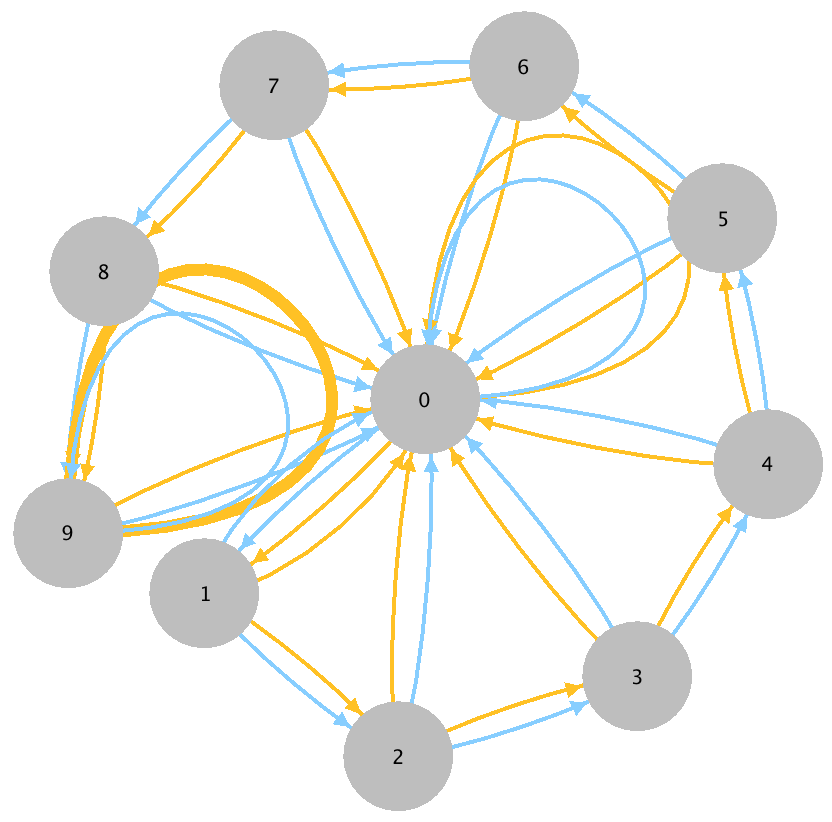
\includegraphics[width=0.42\columnwidth]{figures/ground_nchain_small.png}}
%\subfigure[Abstract NChain]{
%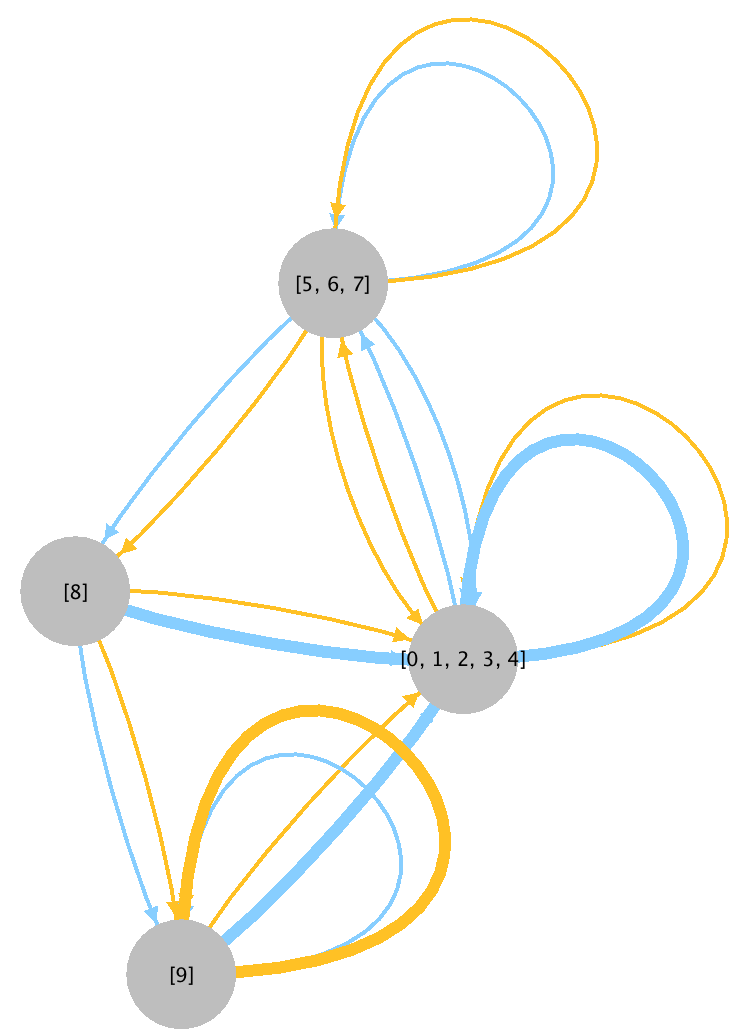
\includegraphics[width=0.42\columnwidth]{figures/abs_nchain.png}}
%\label{fig:nchain-visual}
%\caption{Comparison of ground NChain \ac{MDP} and abstract NChain \ac{MDP}, under an $\epQ$ abstraction, with $\varepsilon=0.5$}
%\end{figure} 

%% Subsection: UpWorld.
%\subsection{UpWorld}
%
%The UpWorld task is an $N\times M$ grid in which the agent starts in the lower left corner. The agent may move left, right, and up. The agent receives positive reward for transitioning to a state at the top of the grid, where moving up in the top cells self transitions. the agent receives 0 reward for all other transitions. Consequently, moving up is always the optimal action, since moving left and right does not change the agent's manhattan distance to positive reward. During experimentation, we set $N=10$, $M=4$.
%
%\begin{figure}
%\subfigure[Ground UpWorld]{
%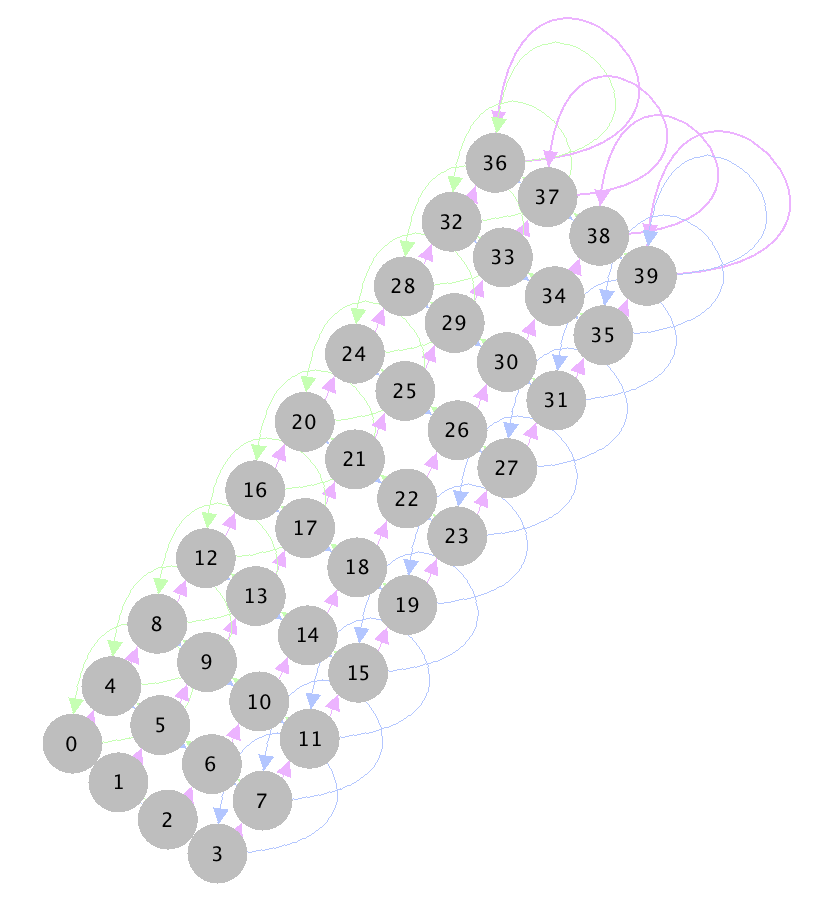
\includegraphics[width=0.48\columnwidth]{figures/ground_upworld.png}}
%\subfigure[Abstract UpWorld]{
%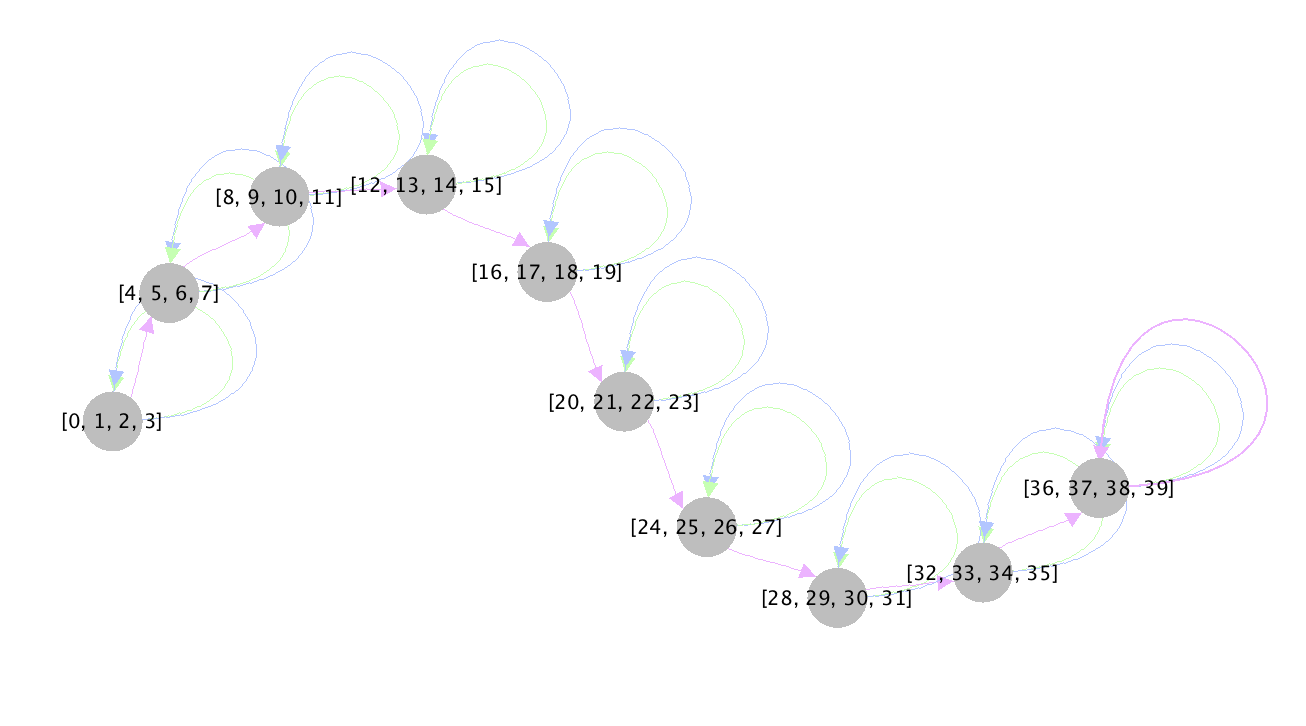
\includegraphics[width=0.48\columnwidth]{figures/abs_upworld.png}}
%\label{fig:upworld-visual}
%\caption{Comparison of Original UpWorld MDP and Abstract MDP, under $\epQ$, with $\varepsilon=0.5$}
%\end{figure} 

% Subsection: Taxi
%\subsection{Taxi}

Taxi has long been studied by the hierarchical RL literature~\cite{dietterich2000hierarchical}. The agent, operating in a grid-world style domain, may move left, right, up, and down, as well as pick up a passenger and drop off a passenger. The goal is achieved when the agent has taken all passengers to their destinations.

%We visualize the compression on a simple 626 Taxi instance in Figure~\ref{fig:taxi-visual}. As stated above, we visualize the original Taxi problem into a graph representation so that we may visualize both the ground MDP and abstract MDP in the same format.

% Taxi Compression Visuals
%\begin{figure}[h]
%\subfigure[Ground Taxi]{
%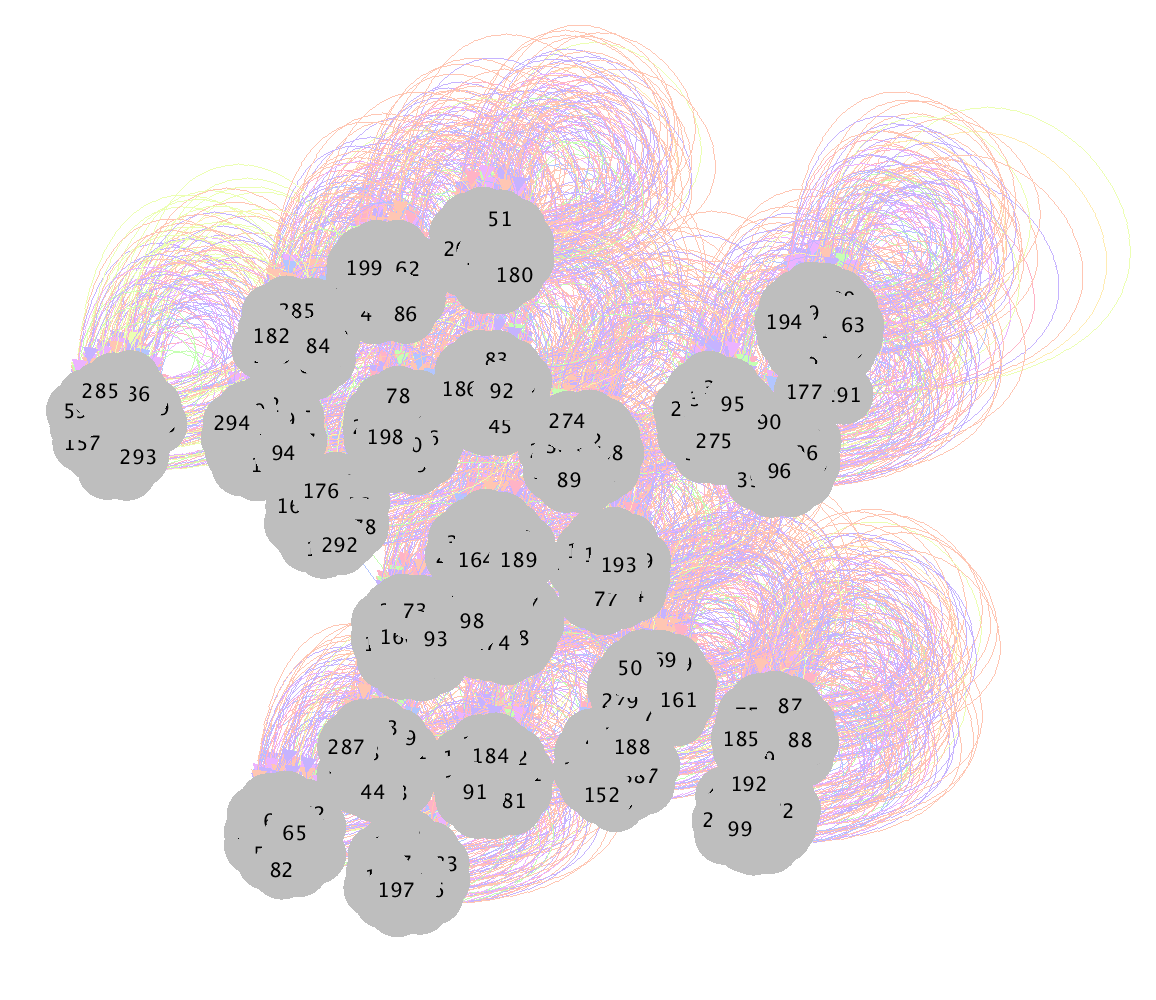
\includegraphics[width=0.48\columnwidth]{figures/ground_taxi.png}}
%\subfigure[Abstract Taxi]{
%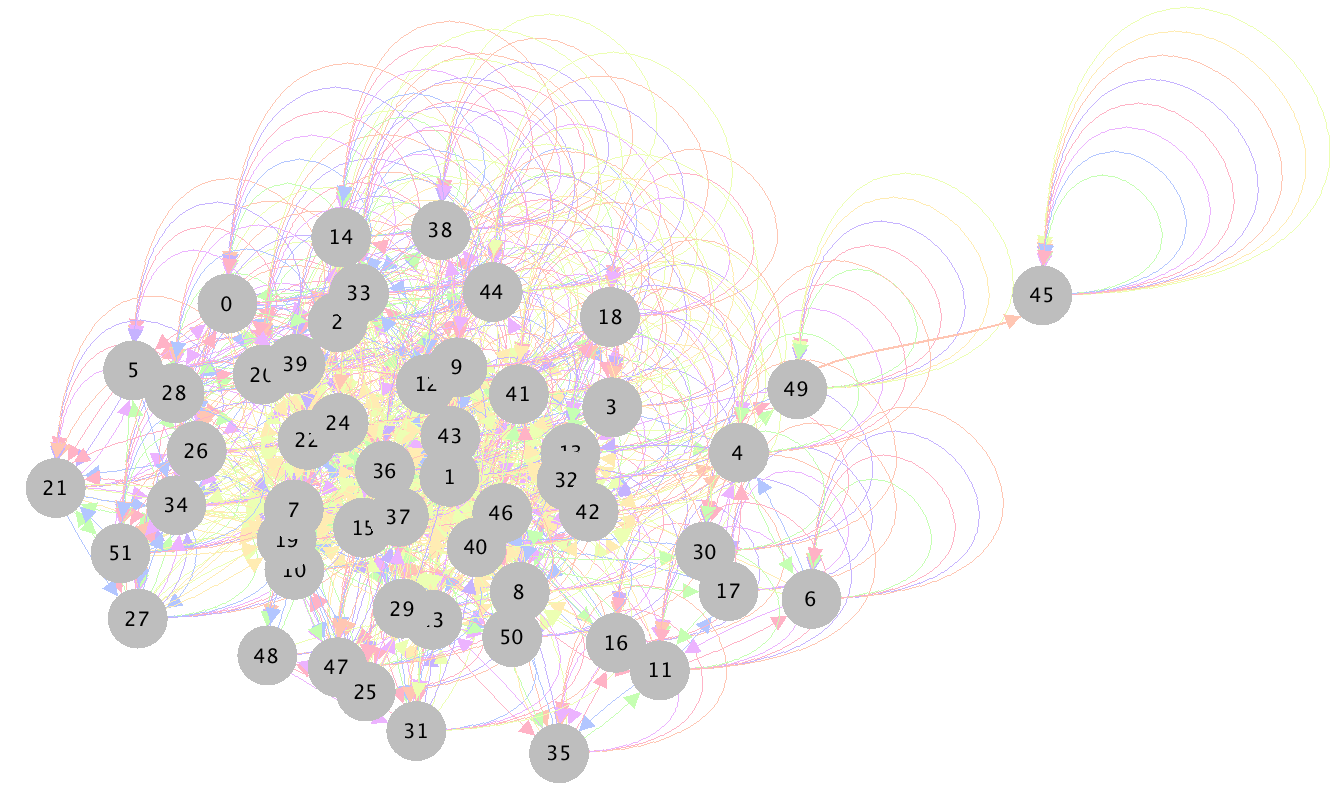
\includegraphics[width=0.48\columnwidth]{figures/abs_taxi.png}}
%\label{fig:taxi-visual}
%\caption{Comparison of Original Taxi MDP and Abstract Taxi MDP, under an $\epQ$ abstraction, with $\varepsilon=0.03$}
%\end{figure} 


% Insert visual and/or stats on number of states and performance of VI solving the abstract MDP and evaluating the resulting policy on the original MDP


% Subsection: Minefield.
%\subsection{Minefield}
Minefield is a test problem we are introducing that uses the Grid World dynamics of \citeauthor{russell1995modern} with slip probability of $x$. The reward function is such that moving up in the top row of the grid receives $1.0$ reward; all other transitions receive $0.2$ reward, except for transitions to a random set of $\kappa$ states (which may include the top row) that receive $0$ reward. (These are the states with ``mines'' in them.) We set $N=10, M=4, \varepsilon=0.5, \kappa = 5, x = 0.01$. We depict the original Minefield and an abstract Minefield in Figure~\ref{fig:minefield-visual}.

% Minefield Compression Visuals
\begin{figure}
\centering
\subfigure[Ground Minefield]{
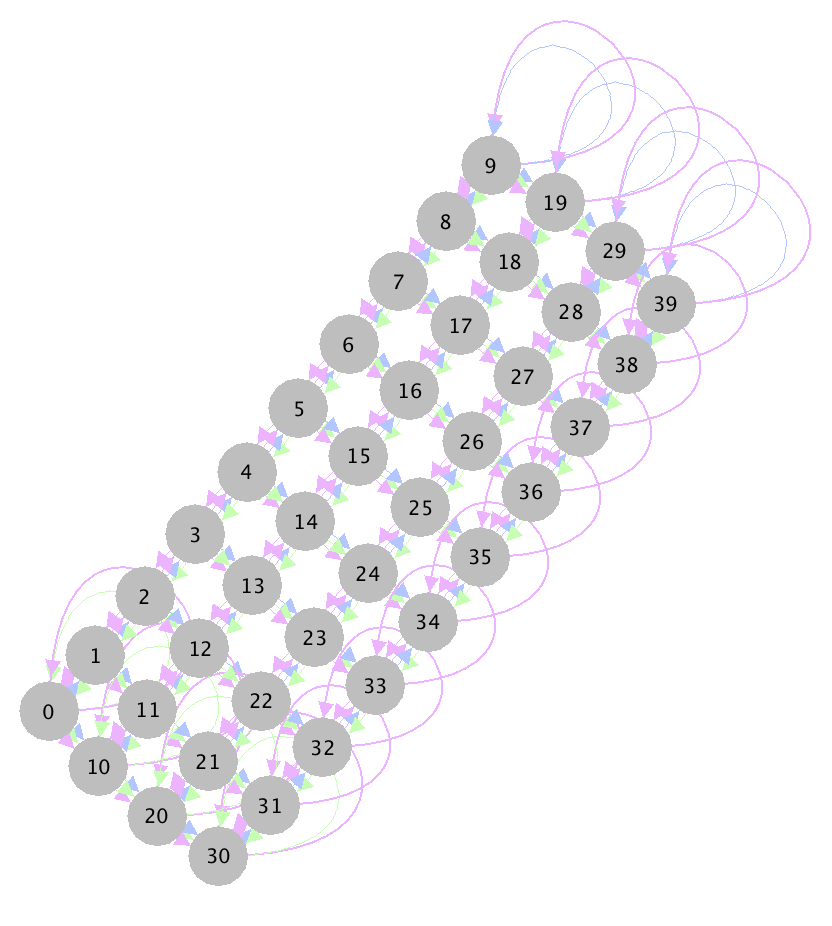
\includegraphics[width=0.4\columnwidth]{figures/ground_minefield.png}}
\subfigure[Abstract Minefield]{
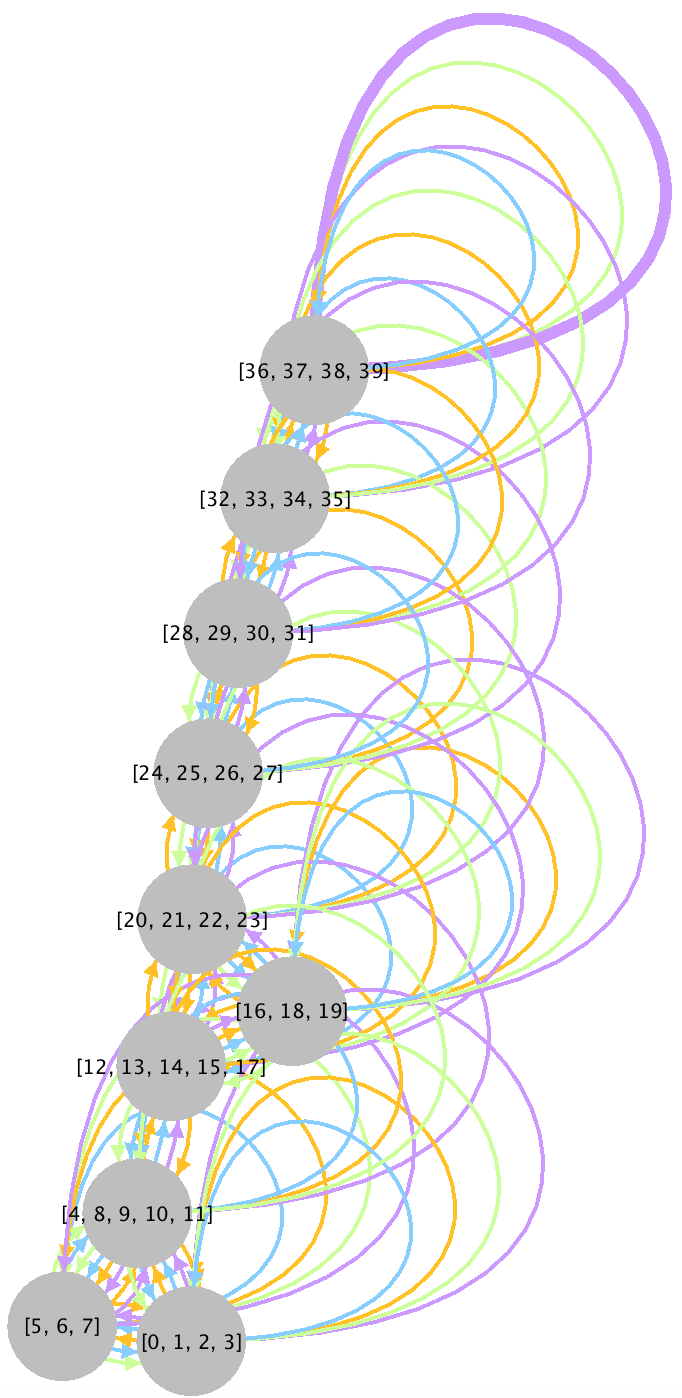
\includegraphics[width=0.4\columnwidth]{figures/abs_minefield.png}}
\label{fig:minefield-visual}
\caption{Comparison of ground Minefield \ac{MDP} and abstract \ac{MDP}, under a $\epQ$ abstraction with $\varepsilon=0.5$}
\end{figure} 

% Subsection: Random.
%\subsection{Random}

In the Random \ac{MDP} domain we consider, there are $100$ states and $3$ actions. For each state, each action transitions to one of two randomly selected states, probability $0.5$.

%The Random MDP and its compression are visualized in Figure~\ref{fig:minefield-visual}.

% Random Compression Visuals
%\begin{figure}
%\subfigure[Ground Random]{
%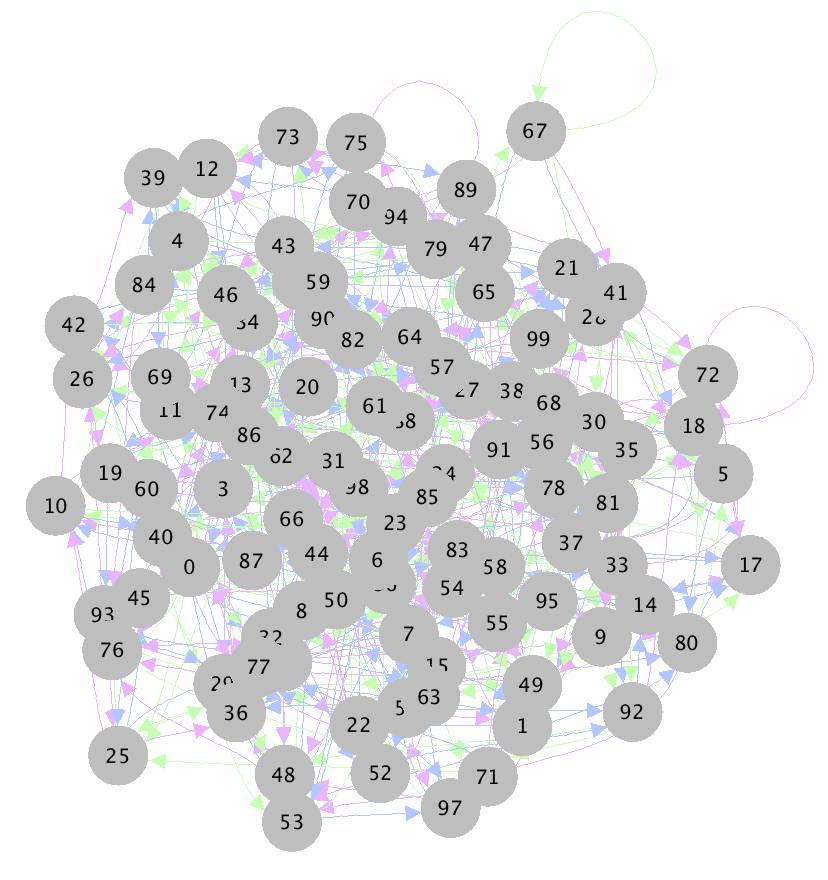
\includegraphics[width=0.48\columnwidth]{figures/ground_random.png}}
%\subfigure[Abstract Random]{
%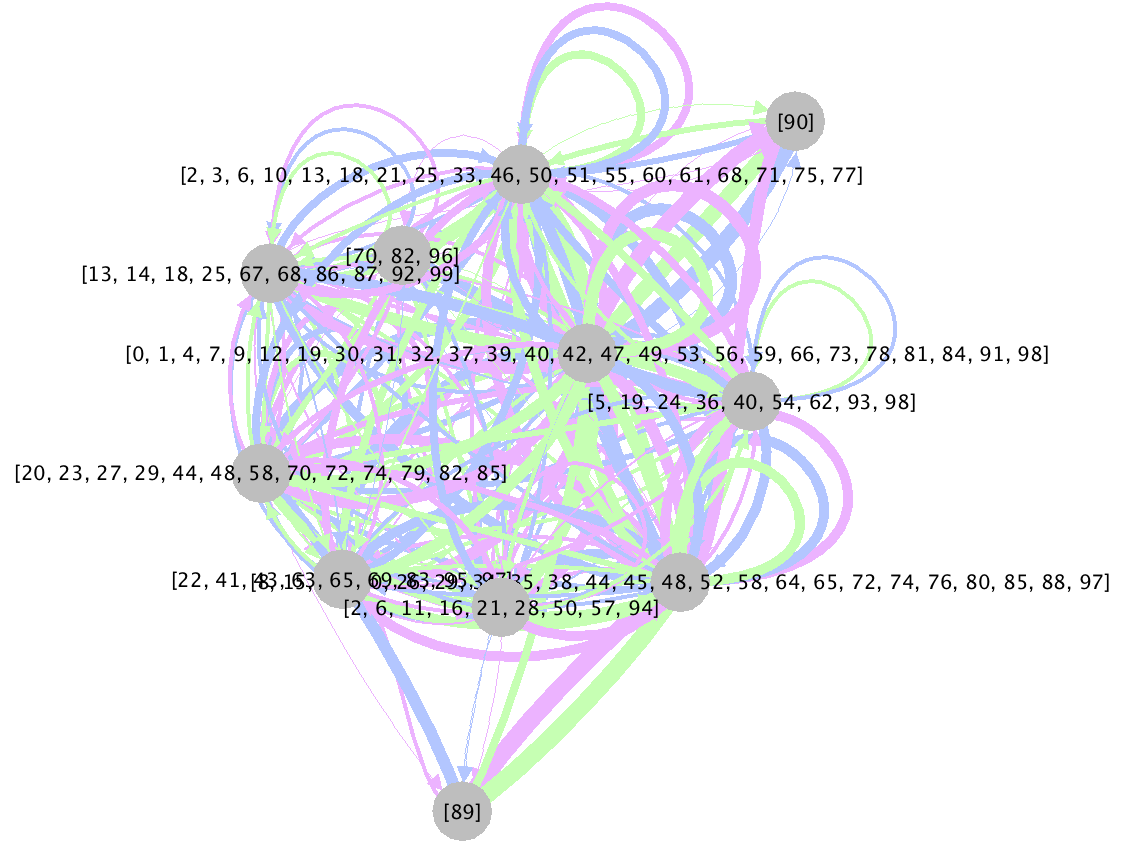
\includegraphics[width=0.48\columnwidth]{figures/abs_random.png}}
%\label{fig:minefield-visual}
%\caption{Comparison of Original Random MDP and Abstract Random MDP, under an $\epQ$ abstraction, with $\varepsilon=0.2$}
%\end{figure} 




% ------------------------------------------------------------------------------------
% --- SECTION: Approximate Abstraction on Example Domains ---s
% ------------------------------------------------------------------------------------
\section{Approximate Abstraction on Example Domains}
%Explanation of what abstraction is used
We run experiments on aggregation functions in the $\epQ$ family of approximate abstractions. For each trial our aggregation greedily groups ground states into abstract states that in a way that satisfies the $\epQ$ criteria. The order in which ground states are grouped is randomized, so there is randomization across trials. Every ground state is equally weighted in its abstract state.

%Explanation of what plots done
For each domain we report two quantities as a function of epsilon with 95\% confidence bars. First, we compare the number of states in the abstract \ac{MDP} for different values of $\epsilon$, shown in Figure~\ref{fig:main_empirical_results1}. The smaller the number of abstract states, the smaller the state space of the $\ac{MDP}$ that the agent must plan over. Second, we report the value under the abstract policy of the initial ground state, shown in Figure~\ref{fig:main_empirical_results2}. In the Taxi and Random domains, 200 trials are run for each data point, whereas 20 trials are run for data points in Minefield and NChain.

%Discuss results
\enote{Make sure results discussion is consistent with "the thesis of this work..."}

Our empirical results corroborate our thesis -- that approximate state abstractions can form the basis of learnable and useful state aggregation criteria. In both NChain and Minefield, we observe that as $\epsilon$ increases from $0$, the number of states which must be planned over is reduced, and optimal behavior is either fully maintained (NChain) or very nearly maintained (Minefield). Similarly for Taxi, when $\epsilon$ is between $.02$ and $.025$ we observe a reduction in the number of states in the abstract \ac{MDP} while value is fully maintained. After $.025$, increased reduction in state space size comes at a cost of value. Lastly, as $\epsilon$ is increased in the Random domain, there is a smooth reduction in the number of abstract states with a corresponding cost in the value of the derived policy.

Our experimental results also highlight a noteworthy characteristic of approximate state abstraction in goal-based \acp{MDP}. Taxi exhibits relative stability in state space size and behavior for epsilon up to $.02$ until both fall off dramatically. We attribute the sudden fall off of these quantities to its goal-based nature; once information critical for achieving optimal behavior is lost in the state aggregation, solving the goal -- and so acquiring any reward -- is unattainable. Conversely, in the Random domain, a great deal of near-optimal policies are available to the agent. Thus, even the information for optimal behavior is lost with an increase in $\epsilon$ there are a great deal of near-optimal policies available to the agent which are not lost by the abstraction.

% Figure: Epsilon vs. #States and Epsilon vs Abstract Pol. For NChain and Minefield.
\begin{figure}
\label{fig:main_empirical_results1}
\centering

\subfigure[NChain]{
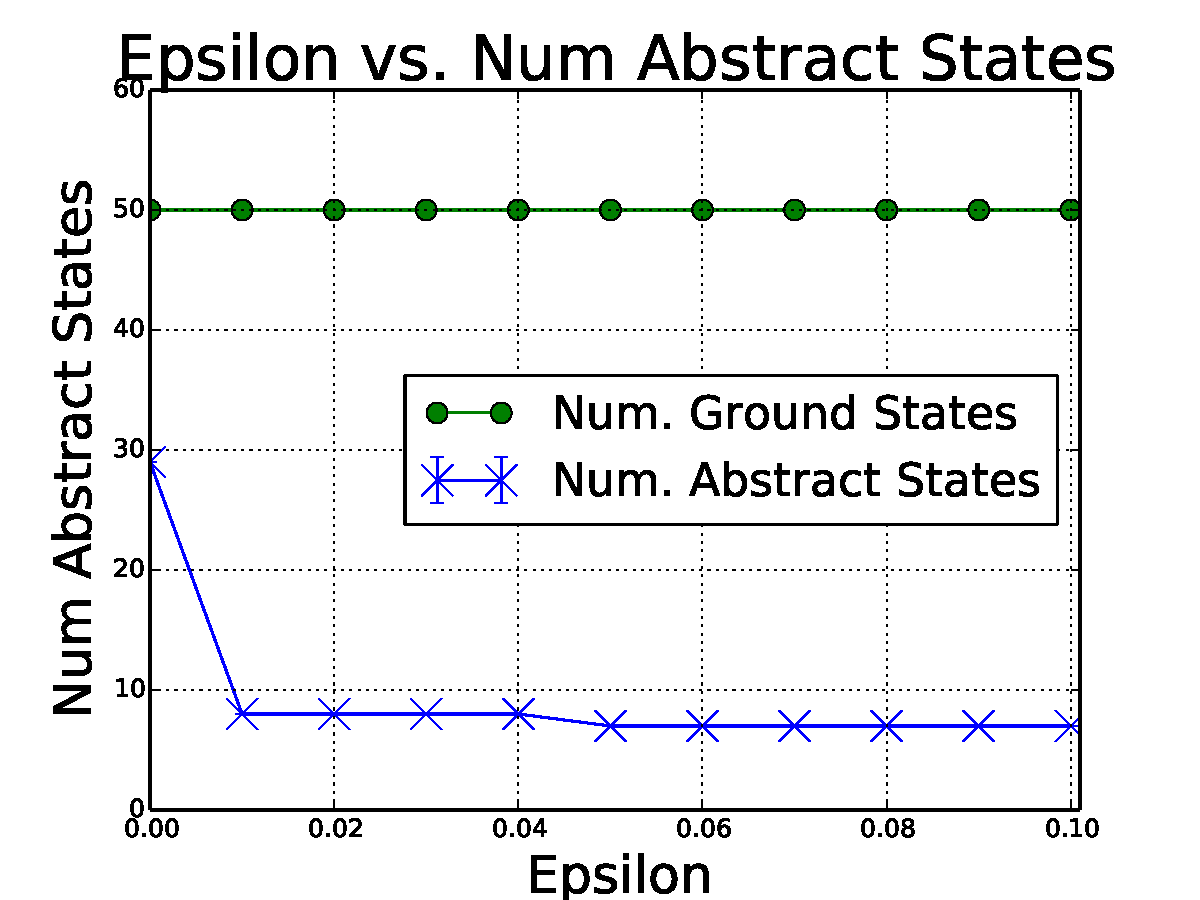
\includegraphics[width=0.46\columnwidth]{figures/nchain_epsilon_vs_num_abstract_states.pdf}
}
\subfigure[NChain]{
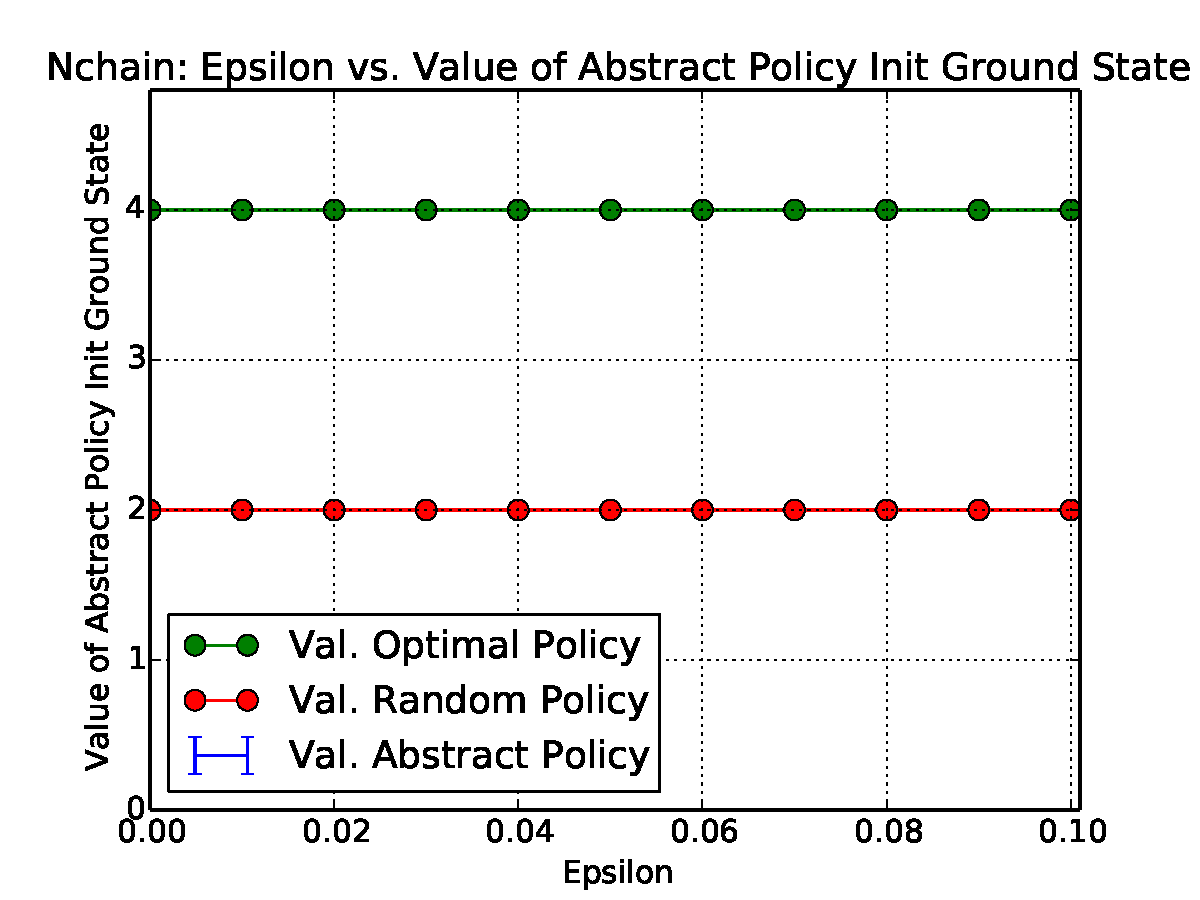
\includegraphics[width=0.46\columnwidth]{figures/nchain_epsilon_vs_value_of_abstract_policy_init_ground_state.pdf}
}

\subfigure[Minefield]{
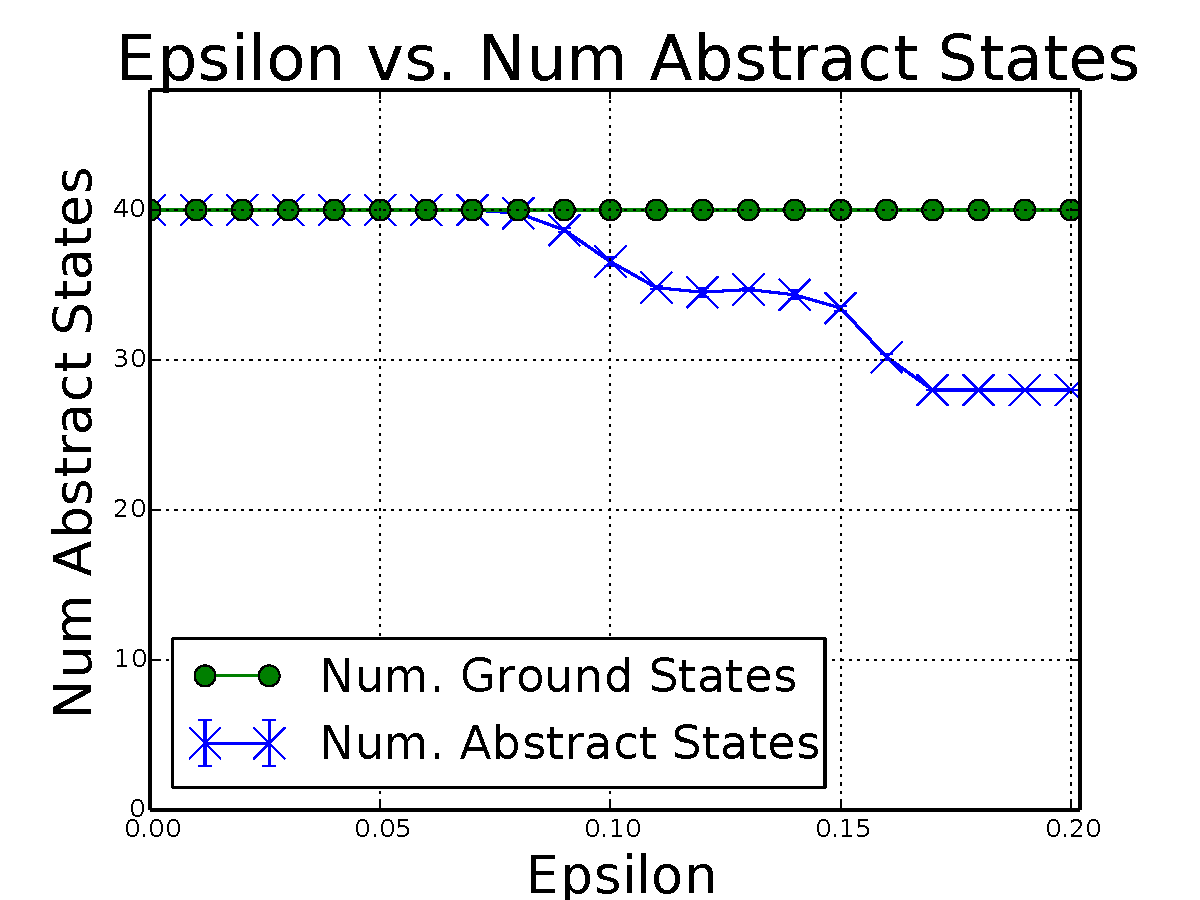
\includegraphics[width=0.46\columnwidth]{figures/minefield_epsilon_vs_num_abstract_states.pdf}
}
\subfigure[Minefield]{
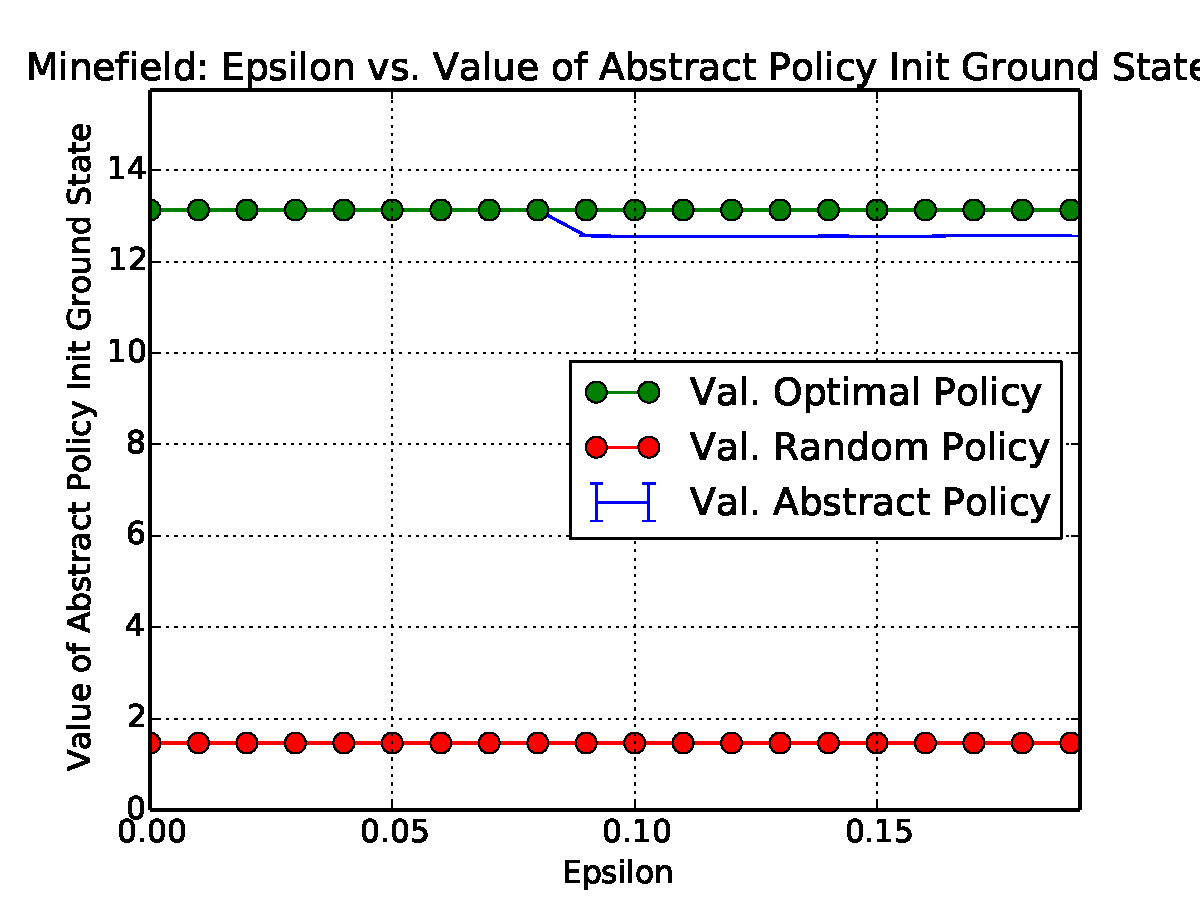
\includegraphics[width=0.46\columnwidth]{figures/minefield_epsilon_vs_value_of_abstract_policy_init_ground_state.pdf}
}

\caption{$\epsilon$ vs. Num States and $\epsilon$ vs. Abstract Policy Value}
\end{figure} 

% Figure: Epsilon vs. #States and Epsilon vs Abstract Pol. For Taxi and Random.
\begin{figure}
\label{fig:main_empirical_results2}
\centering
\subfigure[Taxi]{
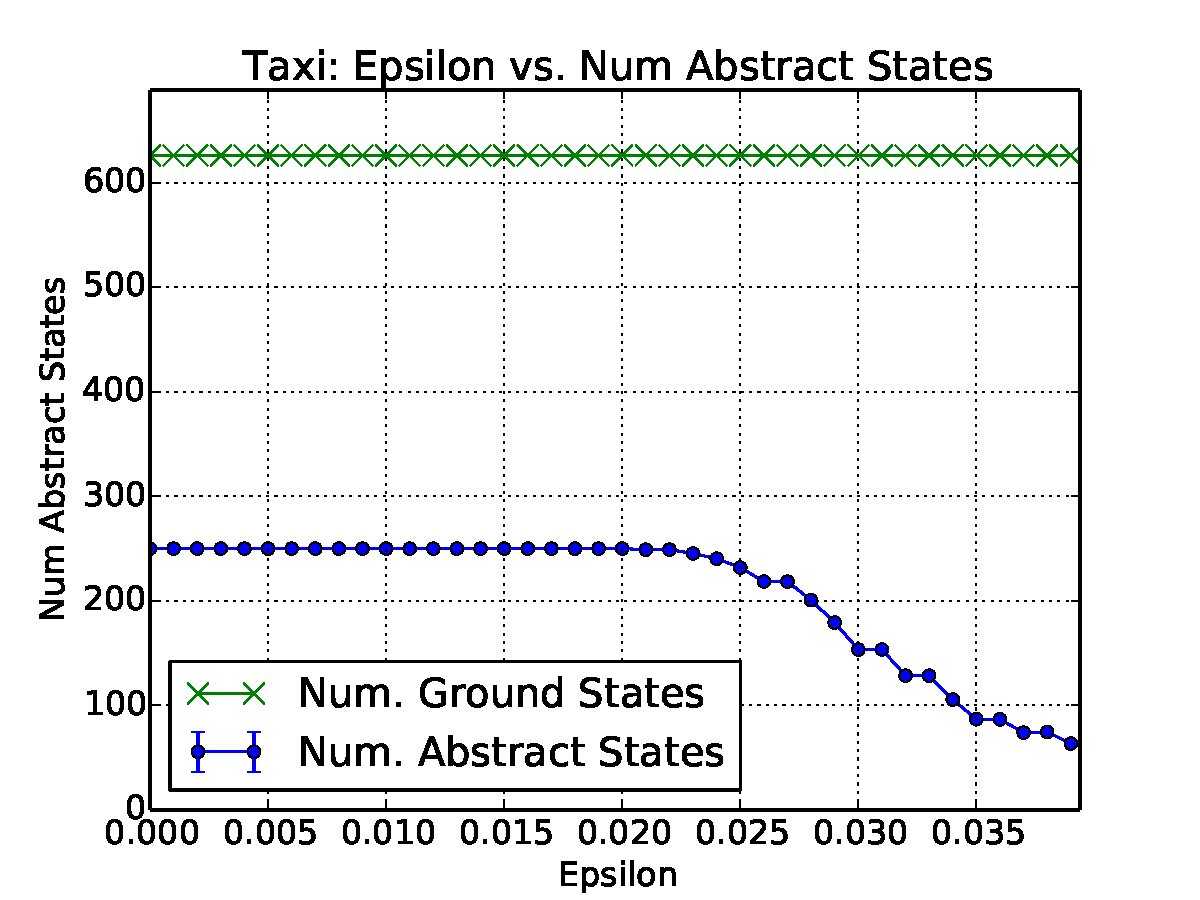
\includegraphics[width=0.46\columnwidth]{figures/taxi_epsilon_vs_num_abstract_states.pdf}
}
\subfigure[Taxi]{
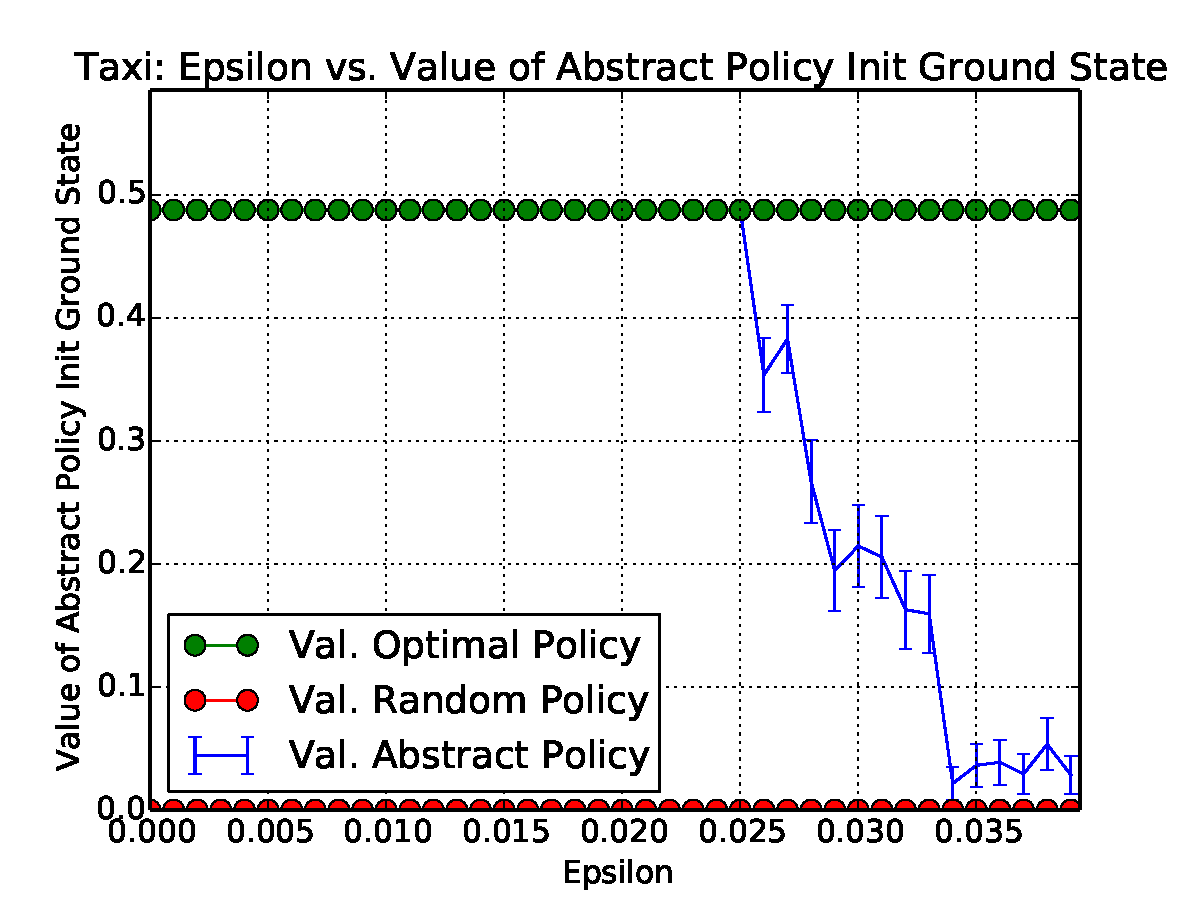
\includegraphics[width=0.46\columnwidth]{figures/taxi_epsilon_vs_value_of_abstract_policy_init_ground_state.pdf}
}

\subfigure[Random]{
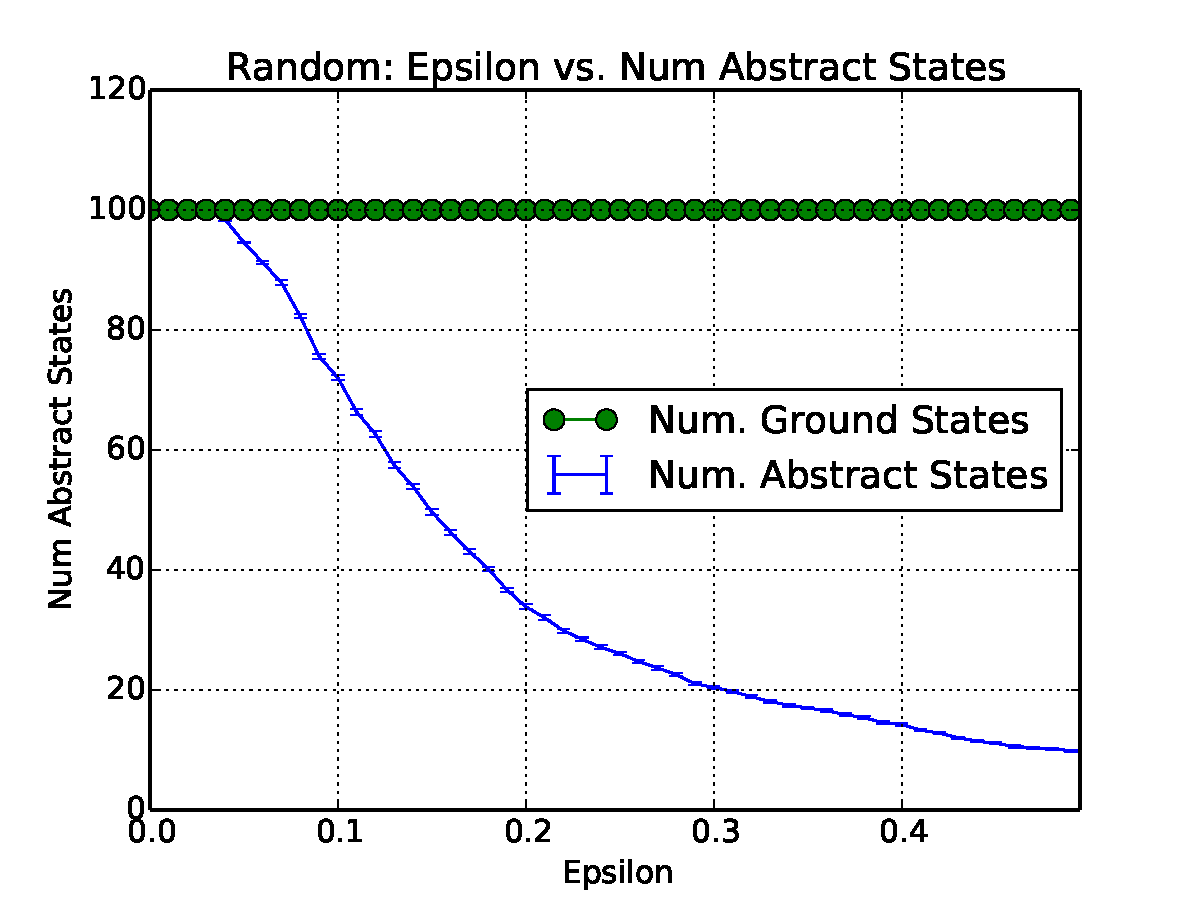
\includegraphics[width=0.46\columnwidth]{figures/random_epsilon_vs_num_abstract_states.pdf}
}
\subfigure[Random]{
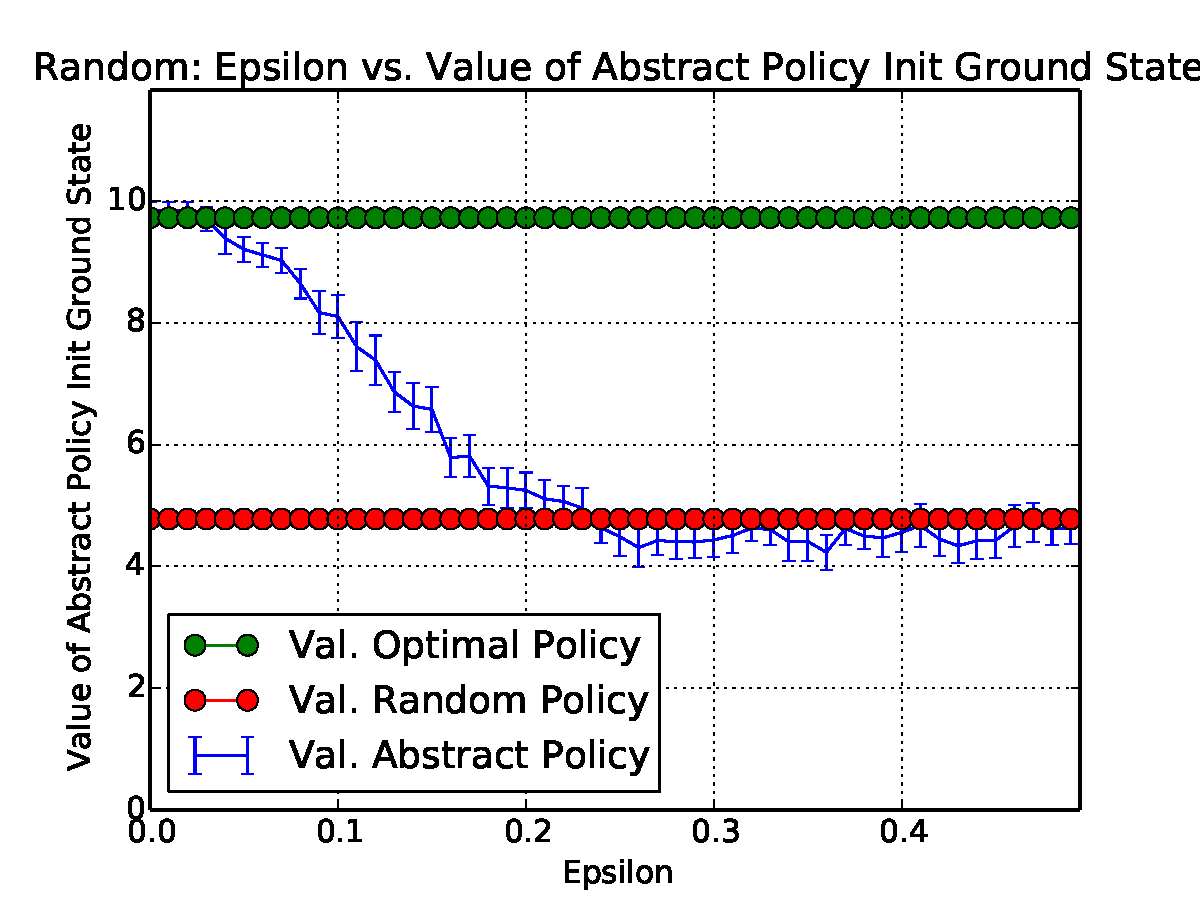
\includegraphics[width=0.46\columnwidth]{figures/random_epsilon_vs_value_of_abstract_policy_init_ground_state.pdf}
}

\caption{$\epsilon$ vs. Num States and $\epsilon$ vs. Abstract Policy Value}
\end{figure} 




% --------------------------------------
% --- SECTION: Conclusion ---
% --------------------------------------
\section{Conclusion}

% Summary of contributions.
Approximate abstraction in \acp{MDP} offers considerable advantages over exact abstraction. In this work, we proved bounds for the value lost when behaving according to the optimal policy of the abstract \ac{MDP}. We also empirically demonstrate that approximate abstractions can reduce state space size with negligible loss in the quality of the behavior.

%First, approximate abstraction relies on criteria that we imagine a planning or learning algorithm to be able to learn without solving the full \ac{MDP}. Second, approximate abstractions can achieve greater degrees of compression due to their relaxed criteria of equality. Third, methods that employ approximate aggregation techniques are able to tune the aggressiveness of abstraction all the while incurring bounded error. We empirically demonstrate the relationship between $\varepsilon$ and the degree of compression, as well as the value of the abstract policy on four dramatically different \acs{MDP}. We provide a code base that provides implementations to abstract, visualize, and evaluate an arbitrary MDP to promote further investigation into approximate abstraction.

% Future work.
There are many directions for future work.
% Learning abs functions online.
First, we are interested in extending the approach of \citet{ortner2013adaptive} by learning the approximate abstraction functions introduced in this paper online in the planning or \ac{RL} setting.
% Necessary conditions.
While our work presents several sufficient conditions for achieving bounded error of learned behavior with approximate abstractions, we hope to investigate what conditions are strictly necessary for an approximate abstraction to achieve bounded error.
% Options/termporal abstraction
We investigated the use of options~\cite{sutton1999between} in the Taxi domain, and found a negligible difference in the degree and quality of compression compared to compression without options. In the future, we are interested in characterizing the relationship between temporal abstractions, such as those afforded by options, and approximate abstractions.
% Compressibility
Lastly, we are interested in understanding the relationship between various approximate abstractions and the information theoretical limitations on the degree of abstraction achievable in \acp{MDP}.

% Exploration is interesting.
%Learning abstraction functions online also has interesting implications for the exploration problem. If certain information informs the agent's ability to abstract more quickly, then exploration directed at learning the abstraction function introduces a new notion of exploration, as an abstraction function will enable the agent to identify near-optimal behavior more quickly, 





% --- BIBLIOGRAPHY ---
\bibliographystyle{icml2016/icml2016}
\bibliography{state_abs}

\end{document}
